%%%%%%%%%%%%%%%%%%%%%%%%%%%%%%%%%%%%%%%%%%%%%%%%%%%%%%%
% A template for Wiley article submissions.
% Developed by Overleaf. 
%
% Please note that whilst this template provides a 
% preview of the typeset manuscript for submission, it 
% will not necessarily be the final publication layout.
%
% Usage notes:
% The "blind" option will make anonymous all author, affiliation, correspondence and funding information.
% Use "num-refs" option for numerical citation and references style.
% Use "alpha-refs" option for author-year citation and references style.

\documentclass[alpha-refs]{wiley-article}

% Add additional packages here if required
\usepackage{multirow}
\usepackage{gensymb}

\usepackage[modulo]{lineno}
\usepackage{setspace}
\onehalfspacing

%\geometry{margin=2cm}

% Guidelines: https://rmets.onlinelibrary.wiley.com/hub/journal/10970088/about/author-guidelines

% Update article type if known
\papertype{Research Article}

\title{Analog Methods and ERA5: Benefits and Pitfalls}

% List abbreviations here, if any. Please note that it is preferred that abbreviations be defined at the first instance they appear in the text, rather than creating an abbreviations list.
\abbrevs{AMs, analog methods; NWP, Numerical weather prediction; CP, calibration period; VP, validation period; AP, archive period}

% Include full author names and degrees, when required by the journal.
% Use the \authfn to add symbols for additional footnotes and present addresses, if any. Usually start with 1 for notes about author contributions; then continuing with 2 etc if any author has a different present address.
\author[1]{Pascal Horton}

% Include full affiliation details for all authors
\affil[1]{Oeschger Centre for Climate Change Research and Institute of Geography, University of Bern, Bern, Switzerland}

\corraddress{Pascal Horton, Oeschger Centre for Climate Change Research and Institute of Geography, University of Bern, 3012 Bern, Switzerland}
\corremail{pascal.horton@giub.unibe.ch}

%\presentadd[\authfn{2}]{Department, Institution, City, State or Province, Postal Code, Country}

%\fundinginfo{Funder One, Funder One Department, Grant/Award Number: 123456, 123457 and 123458; Funder Two, Funder Two Department, Grant/Award Number: 123459}

% Include the name of the author that should appear in the running header
\runningauthor{P. Horton}

\begin{document}

\maketitle

\begin{abstract}
Perfect prognosis statistical downscaling relies on the statistical relationships established using observational data for predictands and predictors. Predictors are often retrieved from reanalyses, which are considered pseudo-observations. The impact of the choice of a reanalysis dataset on the performance of the downscaling method is usually overlooked, as global reanalyses are frequently assumed to be equivalent for the last few decades and data-rich regions such as Europe. However, it was recently shown that the reanalysis dataset can have a bigger impact on the method skill than the choice of predictor variables. Generally, reanalyses processed by more recent atmospheric models assimilate more data and perform best.

This work is aimed at assessing the extent of potential gains from the use of ERA5, following its release, compared to other global reanalyses. The assessment was carried out using six variants of analog methods, which are statistical downscaling techniques, to predict daily precipitation at 301 stations across Switzerland. ERA5 proved to be one of the best performing reanalyses across the different analog methods. Due to data availability, we recommend using 20CR for applications starting between 1851 and 1900, CERA-20C for those between 1900 and 1950, and ERA5 for applications after 1950.

However, ERA5 high spatial resolution (0.25\degree) turned out to be a trap for simple calibration techniques. The domains over which the predictor fields are compared need to be optimized, and high-resolution grids come along with numerous sub-optimal local solutions. An enhanced calibration procedure, thus, must be used. Besides the risk of poorly-calibrated domains, the high resolution also requires much higher computational time with no gain in skill, provided that the predictors considered are relevant at a synoptic scale. Although ERA5 should be the dataset of choice, its use at a lower resolution to predict daily precipitation should provide equivalent performance.


% Please include a maximum of seven keywords
\keywords{Reanalyses, ERA5, Statistical downscaling, Analog methods, Precipitation, Switzerland}

\end{abstract}

\linenumbers

\section{Introduction}

Analog methods (AMs) are statistical downscaling techniques that predict local meteorological variables, often daily precipitation, based on large-scale predictors. AMs rely on the assumption that similar synoptic situations are likely to result in similar local effects plus some variability that cannot be explained by the considered predictors \citep{Lorenz1969}. To account for this unexplained variability, an ensemble of analog situations is considered. It thus provides a statistical prediction in the form of an empirical conditional distribution made from the corresponding observed predictand values. Multiple variants of the AM with different structures, approaches, and -- mainly -- different predictors, exist.

Applications of AMs consist of, for example, daily precipitation predictions, either in an operational forecasting context \citep[e.g.][]{Bontron2005, Hamill2006, Bliefernicht2010, Marty2012, Horton2012, Hamill2015, BenDaoud2016} or for downscaling climate models \citep[e.g.][]{Zorita1999, Wetterhall2005, Wetterhall2007, Matulla2007, Radanovics2013, Chardon2014, Dayon2015, Raynaud2016b}. Other applications target precipitation radar images \citep{Panziera2011, Foresti2015a}, temperature \citep{Kruizinga1983, DelleMonache2013, Caillouet2016, Raynaud2016b}, wind \citep{DelleMonache2013, DelleMonache2011, Vanvyve2015, Alessandrini2015, Junk2015, Junk2015c}, solar radiation or power production \citep{Alessandrini2015a, Bessa2015, Raynaud2016b}, and the trajectory of tropical cyclones \citep{Sievers2000, Fraedrich2003}. AMs are also used for seasonal forecast \citep{Xavier2007, Charles2012, Wu2012, Shao2013}.

AMs are most often developed in a perfect prognosis framework \citep{Rummukainen1997, Maraun2010}, where the statistical relationship is calibrated between large-scale and local-scale observations. In this context, global reanalyses are the datasets of choice for large-scale variables as they provide multivariate gridded outputs that are physically consistent and available all around the globe \citep{Gelaro2017}. Once the relationship has been established (i.e., the predictor variables selected and the other parameters calibrated), the AM is then applied in a different context, such as forecasting, climate reconstruction, or climate projections. In such contexts, precipitation is predicted using the target model output to describe the target situation for the AM and the reanalysis dataset as the archive to retrieve past analog situations (if no long reforecast dataset is available). Globally, two main types of reanalysis products exist: those that aim for homogeneity over a long period -- starting at the beginning of the 20th century -- and hence assimilate surface data only, and those that aim for accuracy over a more recent period (typically 1979) and therefore assimilate as many observations as possible, including multiple satellite products. The reanalyses accuracy depends on the quality of the model physics and the analysis process, as well as the quantity and quality of the assimilated observations \citep{Dee2011a}.

The nature of the application can drive the choice of a reanalysis dataset for AMs. For example, if a coverage of the 20th century is needed, the Twentieth Century Reanalysis produced by the European Centre for Medium-Range Weather Forecasts (ECMWF) \citep[ERA-20C or CERA-20C --][]{Poli2016, Laloyaux2016} or 20CR \citep{Compo2011} produced by NOAA -- now available as version 3 \citep{Slivinski2019, Slivinski2021} -- can be used \citep[for example,][]{Kuentz2015, Caillouet2016, Brigode2016, Bonnet2017}. In an operational forecasting context, with the target situation being provided by an NWP model, one should prefer a reanalysis that is produced by the same NWP model as the operational forecast to reduce inter-model biases. However, in many cases, the selection of the reanalysis is arbitrary and might be driven by a preference for the local provider.  

NCEP/NCAR Reanalysis 1 \citep[NR-1 --][]{Kalnay1996, Kistler2001} and NCEP/DOE Reanalysis 2 \citep[NR-2 --][]{Kanamitsu2002} were used in many AM applications \citep[e.g.][]{Timbal2003, Altava-Ortiz2006, Matulla2007, Yiou2014}. ERA-40 \citep{Uppala2005}, produced by ECMWF, has also been used substantially \citep[e.g.][] {Willems2011b, Radanovics2013, Chardon2014, BenDaoud2016}. Its sucessor, ERA-Interim \citep[ERA-INT --][]{Dee2011a}, has been used by \cite{Raynaud2016b}. NASA's Modern-Era Retrospective Analysis for Research and Applications \citep[MERRA -- ][]{Rienecker2011} has been used by \citet{Vanvyve2015}. The Japanese 55-year Reanalysis \citep[JRA-55 --][]{Kobayashi2015, Harada2016} and its conventional-data-only JRA-55 Conventional \citep[JRA-55C --][]{Kobayashi2014}, have not been used in AMs to the author’s knowledge. Newer products, such as NCEP's Climate Forecast System Reanalysis \citep[CFSR --][]{Saha2010a}, MERRA version 2 \citep[MERRA-2 -- ][]{Gelaro2017} or ERA5 \citep{Hersbach2020} have not been used much in AMs. This is the result of the lag one often observes between the release of a new reanalysis dataset and its adoption in AMs.

Most AM applications are based on a single reanalysis dataset and its impact is overlooked. \citet{BenDaoud2009} compared NR-1 with ERA-40 and found no significant difference for the predictors considered. Later, \citet{Dayon2015} compared NR-1, MERRA, ERA-INT, and 20CR, and found that the choice of the reanalysis dataset has a non-negligible impact on the performance of AMs. This impact can even be greater than that of the choice of the predictor variables. It was concluded that the role of the reanalyses should not be underestimated. Such influence has also been observed for other statistical downscaling methods \citep[e.g.][]{Koukidis2009}. \citet{Horton2018b} compared ten global reanalyses and concluded that the impact of the dataset on the results of the AM is significant. Similarly to the work of \citet{Dayon2015}, the impact of the reanalysis was sometimes found to be higher than that of the selected predictors. 

Generally, more recent products that assimilate more data and come with a higher spatial resolution result in better predictions in AMs \citep{Horton2018b}. However, this is not systematically the case as, for example, JRA-55, which has a lower spatial resolution (1.25\degree), was found to be one of the best options for more complex AMs. Moreover, the choice of a reanalysis can be driven by the period of interest. As there was no better dataset overall, a table has been provided by \citet{Horton2018b} for guidance in the selection of a reanalysis for a given predictor and period. Some characteristics of the datasets were also assessed, such as the spatial resolution, archive length, and use of ensemble members. For most AMs and datasets, there was a gain in skill with increasing resolution up to 1\degree; below this, however, the gains were almost null. The use of long archives for reanalyses with extended data improved the performance to some extent by providing potentially better analog situations, particularly for less frequent situations. However, former times were more data-scarce and data might be inhomogeneous over long periods which can, in turn, have a negative effect on the skill of AMs exploiting these archives \citep{Horton2018b}. Finally, the use of ensemble members showed limited benefits and that great caution is required for their use in methods with multiple levels of analogy.

This work is a follow-up to \citet{Horton2018b} and focuses on ERA5 by comparing its impact on six AMs using nine other major reanalyses at 301 stations in Switzerland. The study of the characteristics of the reanalyses as provided in \citet{Horton2018b} is not repeated here as the conclusions are likely identical. The optimal parameters, such as the number of analogs and the size of the comparison domain, were here compared across reanalyses and discussed. This provides an original insight into the role of the spatial resolution and reanalysis quality. The benefits and potential pitfalls of ERA5’s high spatial resolution are also assessed.

The article is structured as follows: Sect. \ref{sec:data_methods} describes the reanalyses compared in this work, provides some information on the precipitation dataset used and the study period, details the assessed AMs and their calibration. Sect. \ref{sec:results} shows the results. It starts with an analysis of the role of the spatial resolution and the related pitfalls for the calibration procedure (Sect. \ref{sec:results_hires}). A comparison of the AM parameters calibrated for the different reanalyses is then provided (Sect. \ref{sec:results_parameters}). Finally, it shows how ERA5 compares to the other reanalyses (Sect. \ref{sec:results_skill}). The conclusions are provided in Sect. \ref{sec:conclusion}.


\section{Data and methods}
\label{sec:data_methods}

\subsection{Reanalyses}
\label{sec:reanalyses}

The present work aims at comparing ERA5 \citep{Hersbach2020} with other global reanalyses, whose characteristics are provided in Table \ref{table:datasets}, thus complementing the work of \citet{Horton2018b}. The first three reanalyses in Table \ref{table:datasets} are surface-input \citep{Fujiwara2017} products that assimilate surface data only but cover an extended period, typically from the start of 20th century. NOAA produced the Twentieth Century Reanalysis \citep[version 2c, 20CR-2c --][]{Compo2011}, which only assimilates surface pressure data and uses observed monthly sea-surface temperatures and sea-ice distributions as boundary conditions. A more recent version, 20CRv3 \citep{Slivinski2019, Slivinski2021}, has been released since the comparison presented here was performed (and is thus not part of this work). This third version solves issues found in version 2c and was produced using an upgraded data assimilation system as well as a newer forecast model. The ECMWF developed two products using surface input only. The first is ERA-20C \citep{Poli2016}, which assimilates marine wind observations and is forced by sea surface temperature, sea ice cover, atmospheric composition changes, and solar forcing. The second is CERA-20C \citep{Laloyaux2018a}, which has an additional coupling to the ocean and was produced by a more recent version of the Integrated Forecasting System (IFS) model.

The other reanalyses are full-input products that assimilate all available data, including satellite data \citep{Fujiwara2017}. NCEP/NCAR Reanalysis 1 \citep[NR-1 --][]{Kalnay1996, Kistler2001} was the first global reanalysis followed by NCEP/DOE Reanalysis 2 \citep[NR-2 --][]{Kanamitsu2002}, which fixed some identified problems. The Climate Forecast System Reanalysis \citep[CFSR --][]{Saha2010a} is the most recent one produced by the NCEP. The Japanese 55-year Reanalysis \citep[JRA-55 --][]{Kobayashi2015, Harada2016} is produced by the Japan Meteorological Agency (JMA). JRA-55 Conventional \citep[JRA-55C --][]{Kobayashi2014}, which uses conventional data only, was not considered in this work as it provides similar results to JRA-55 \citep{Horton2018b}. NASA's Global Modeling and Assimilation Office (GMAO) released the Modern-Era Retrospective Analysis for Research and Applications version 2 \citep[MERRA-2 -- ][]{Gelaro2017}, which is an improvement on the first MERRA reanalysis \citep{Rienecker2011}. Finally, the predecessor of ERA5, ERA-Interim \citep[ERA-INT --][]{Dee2011a}, was also considered.

ERA5 \citep{Hersbach2020} is meant to replace ERA-Interim. It benefits from multiple improvements to IFS in terms of model physics, core dynamics, and data assimilation \citep{Hersbach2020}. It provides more outputs with higher temporal (hourly) and spatial (0.25\degree) resolutions. It has the highest spatial and temporal resolution to date. The use of a 10-member ensemble of data assimilation at a lower spatial and temporal resolution allows an estimation of its uncertainty. ERA5 assimilates significantly more data than ERA-Interim, such as data from ground-based radar and new satellite sensors, and uses improved observation operators, thus allowing better comparison of model outputs with observations. Additionally, it indirectly benefits from improvements in historical observations of both conventional and satellite data \citep{Hersbach2020}. ERA5 provides, among others, more consistent sea surface temperature and sea ice concentration, an improved representation of tropical cyclones, a better balance of evaporation and precipitation, and improved soil moisture. ERA5 is also more suitable for climate analyses as it relies on appropriate radiative forcing and boundary conditions (e.g., changes in greenhouse gases, aerosols, SST, and sea ice).


\begin{table}[bt]
	\caption{Assessed reanalysis datasets with their respective properties, sorted by type and model age.}
	\small
	\begin{threeparttable}
		\begin{tabular}{lllllll}
			\hline
			\headrow
			\thead{Name} & \thead{Institution} & \thead{Coverage} & \thead{Output} & \thead{Model resolution \& age} & \thead{Input} & \thead{Assimilation}\\
			\hline 
			\textbf{20CR-2c} & NOAA-CIRES & 1851 -- 2014 & 2\degree x 2\degree & T62 ($\sim$1.88\degree), L28, 2008 & surface  & EnKF\\
			\textbf{ERA-20C} & ECMWF & 1900 -- 2010 & 1\degree x 1\degree & TL159 ($\sim$1.13\degree), L9, 2012 & surface  & 4D-Var\\
			\textbf{CERA-20C} & ECMWF & 1901 -- 2010 & 1\degree x 1\degree & T159 ($\sim$1.13\degree), L91, 2016 & surface & 4D-Var\\
			\hline 
			\textbf{NR-1} & NCEP, NCAR & 1948 -- present & 2.5\degree x 2.5\degree & T62 ($\sim$1.88\degree), L28, 1995 & full & 3D-Var\\
			\textbf{NR-2} & NCEP, DOE & 1979 -- present & 2.5\degree x 2.5\degree & T62 ($\sim$1.88\degree), L28, 2001 & full  & 3D-Var\\
			\textbf{CFSR} & NCEP & 1979 -- present & 0.5\degree x 0.5\degree & T382 ($\sim$0.31\degree), L64, 2009 & full  & 3D-Var\\
			\textbf{JRA-55}  & JMA & 1958 -- present & 1.25\degree x 1.25\degree & TL319 ($\sim$0.36\degree), L60, 2009 & full  & 4D-Var\\
			%\textbf{JRA-55C}  & JMA & 1958 -- 2015 & 1.25\degree x 1.25\degree & TL319 ($\sim$0.36\degree), L60 & 2009 & conventional  & 4D-Var\\
			\textbf{MERRA-2} & NASA GMAO & 1980 -- present & 0.625\degree x 0.5\degree & 0.625\degree x 0.5\degree, L72, 2014 & full  & 3D-Var\\
			\textbf{ERA-INT} & ECMWF & 1979 -- 2019 & 0.75\degree x 0.75\degree & TL255 ($\sim$0.70\degree), L60, 2006 & full  & 4D-Var\\
			\textbf{ERA5} & ECMWF & 1950 -- present & 0.25\degree x 0.25\degree & T639 ($\sim$0.28\degree), L137, 2016 & full  & 4D-Var\\
			\hline 
		\end{tabular} 
		
		\begin{tablenotes}
			\item *the data over the period 1950-1978 is only available in a preliminary version at time of writing.
			%\item JKL, just keep laughing; MN, merry noise.
		\end{tablenotes}
	\end{threeparttable}
	\label{table:datasets}
\end{table}


\subsection{Precipitation dataset}
\label{sec:precipitation}

The local variables to be predicted here are daily precipitation totals (06:00~h~UTC to 06:00~h~UTC the following day) at 301 stations of the MeteoSwiss network in Switzerland (Fig. \ref{fig:stations}), with good coverage of the 1981--2010 period. The 30-year precipitation dataset was divided into a calibration period (CP) and an independent validation period (VP) which was evenly distributed over the entire series (1 year out of every 5; a total of 6 years). The archive period (AP), in which the analog dates are being retrieved, is the same as the CP -- also with the VP being excluded -- with an additional exclusion of $\pm30$ days around the target date. The results below are always shown for the VP.


\subsection{Analog methods}
\label{sec:ams}

Most AM variants from the analysis of \cite{Horton2018b} were considered here (Table \ref{table:methods}). These AMs have different degrees of complexity, but they all start with a preselection to cope with seasonality. A commonly used preselection is based on calendar dates (PC: preselection on a calendar-basis in Table \ref{table:methods}) as candidate situations are extracted from the archive for a period of 120~days centered around the target date. To allow for a more dynamic approach, \citet{BenDaoud2016} based this preselection on the similarity of air temperature (T) at 925~hPa and 600~hPa at the nearest grid point. A resulting mixing of spring and autumn situations, which is undesirable, is discussed in \citet{Caillouet2016}. 

\begin{table*}[t]
	\caption{Analogue methods considered in this work, listed by increasing complexity. The analogy criterion is S1 for SLP and Z and RMSE for the other variables.}
	\small
	\begin{threeparttable}
		\begin{tabular}{llllll}
			\hline
			\headrow
			\thead{Method} & \thead{P0} & \thead{L1} & \thead{L2} & \thead{L3} & \thead{Reference} \\ 
			\hline 
			\multirow{2}{*}{\textbf{2Z}} & \multirow{2}{*}{PC} & Z1000@12h &&& \multirow{2}{*}{\citealp{Bontron2004}} \\
			&& Z500@24h &&& \\
			\hline 
			\multirow{4}{*}{\textbf{4Z}} & \multirow{4}{*}{PC} & Z1000@06h &&& \multirow{4}{*}{\citealp{Horton2018a}} \\
			&& Z1000@30h &&& \\
			&& Z700@24h &&& \\
			&& Z500@12h &&& \\
			\hline 
			\multirow{2}{*}{\textbf{2Z-2MI}} & \multirow{2}{*}{PC} & Z1000@12h & \multirow{2}{*}{MI850@12+24h} && \multirow{2}{*}{\citealp{Bontron2004}} \\
			&& Z500@24h &&& \\
			\hline 
			\multirow{4}{*}{\textbf{4Z-2MI}} & \multirow{4}{*}{PC} & Z1000@30h &&& \multirow{4}{*}{\citealp{Horton2018a}}\\
			&& Z850@12h & MI700@24h && \\
			&& Z700@24h & MI600@12h && \\
			&& Z400@12h &&& \\
			\hline 
			\multirow{2}{*}{\textbf{PT-2Z-4MI}} & T925@36h & Z1000@12h & MI925@12+24h && \multirow{2}{*}{\citealp{BenDaoud2016}} \\
			& T600@12h & Z500@24h & MI700@12+24h && \\
			\hline 
			\multirow{2}{*}{\textbf{PT-2Z-4W-4MI}} & T925@36h & Z1000@12h & \multirow{2}{*}{W850@06-24h} & MI925@12+24h & \multirow{2}{*}{\citealp{BenDaoud2016}} \\
			& T600@12h & Z500@24h && MI700@12+24h & \\
			\hline 
		\end{tabular} 
		
		\begin{tablenotes}
			\item P0, preselection (PC: $\pm 60$ days around the target date); L1, L2 and L3, subsequent levels of analogy.
			\item Z, geopotential height; T, air temperature; W, vertical velocity; MI, moisture index (product of the relative humidity at the given pressure level and the total water column).
		\end{tablenotes}
	\end{threeparttable}
	\label{table:methods}
\end{table*}

All considered AMs have a first level of analogy based on the atmospheric circulation, using the geopotential height (Z) at different pressure levels and time as predictor. This analogy is quantified by the S1 criterion \citep[Eq.\ \ref{eq:S1}, ][]{Teweles1954, Brown2012}, which is a comparison of gradients over a selected (calibrated) domain. The S1 criterion allows comparing the atmospheric circulation instead of the absolute values of the respective fields. The S1 values processed for different levels/hours are averaged into a single value. More advanced approaches introduce a weighting between these components \citep{Horton2017a}.

\begin{equation}
	\label{eq:S1}
	S1=100 \frac{\sum_{i} \vert \Delta\hat{z}_{i} - \Delta z_{i} \vert}{\sum_{i} \max\left\lbrace \vert \Delta\hat{z}_{i} \vert; \vert \Delta z_{i} \vert \right\rbrace }
	% use \displaystyle to max sum sign larger
\end{equation}
where $\Delta \hat{z}_{i}$ is the geopotential height gradient between the \textit{i}-th pair of points for the target day and $\Delta z_{i}$ is the corresponding observed geopotential height gradient for the candidate situation. The smaller the value S1 is, the more similar are the pressure fields.

The simplest method, 2Z, is based on the analogy of the atmospheric circulation alone, using the geopotential height at 1000~hPa and 500~hPa \citep{Bontron2004}. The most similar $N_{1}$ dates with the lowest values of S1 are selected as analogs to the target date. The daily precipitation measured on these $N_{1}$ dates then provides the empirical conditional distribution, considered as the probabilistic prediction for the target date.

The second method, 4Z, is also based only on geopotential heights, but it uses four combinations of pressure levels and temporal windows \citep{Horton2018a}. The method considered here is a simplified version of a more sophisticated method elaborated by genetic algorithms. It was found that using four geopotential heights provides more information than using two \citep{Horton2018a}.

The next three methods (2Z-2MI, 4Z-2MI, PT-2Z-4MI, Table \ref{table:methods}) add a second level of analogy based on moisture variables to subsample from the first level. The predictor for this second level of analogy is a moisture index (MI). It is the product of the total precipitable water (TPW) and the relative humidity (RH) and was introduced by \citet{Bontron2004}. This predictor is assessed using the root mean square error (RMSE) criterion. The 2Z-2MI method \citep{Bontron2004} uses this index at 850~hPa for two different hours (+12 h and +24 h). The 4Z-2MI method \citep{Horton2018a}, derived from optimizations with genetic algorithms, uses the moisture index at 600~hPa and 700~hPa, with a change in the selected levels of the geopotential height compared to 4Z. The 4Z-2MI method \citep{BenDaoud2016} considers the moisture index at 700~hPa and 925~hPa, both at +12 h and +24 h.

Finally, the most complex method, PT-2Z-4W-4MI, also named Stepwise Analogue Downscaling Method for Hydrology (SANDHY) \citep{BenDaoud2016, Caillouet2016}, adds an intermediate level of analogy before the moisture predictors, based on the vertical velocity (W) at 850~hPa. It was primarily developed for large and relatively flat/lowland catchments in France (Sa\^{o}ne, Seine).



\subsection{Calibration of the methods} %\subsubsection?
\label{sec:calibration}

The Continuous Ranked Probability Score \citep[CRPS,][]{Brown1974, Matheson1976, Hersbach2000} is often used as the performance metric for AMs as it allows evaluation of the predicted cumulative distribution provided by the analogs with regard to the single observed value on the target date. Its skill score expression, the Continuous Ranked Probability Skill Score (CRPSS), was used here, using the climatological distribution of precipitation at each station as the reference. It allows a better comparison among stations as it takes into account the differences in climatology to some extent. The CRPSS is expressed as follows \citep{Bradley2011}:

\begin{equation}
	\label{eq:CRPSS}
	CRPSS = 1-\frac{\overline{CRPS}}{\overline{CRPS}_{clim}}
\end{equation}
where $CRPS_{clim}$ is the CRPS value for the climatological distribution. A better prediction is characterized by an increase in CRPSS.

The methods were calibrated using the semi-automatic sequential procedure, which was developed by \citet{Bontron2004} and also used in \citet{Radanovics2013} and \citet{BenDaoud2016}. It allows calibrating the spatial windows on which the predictors are compared (specific to each level of analogy) and the number of analog dates for the different levels of analogy. The procedure starts with the calculation of the relevance map, which involves assessing the skill of all points of the predictor grid within a predefined domain. The spatial windows are then calibrated by incremental increases starting from the data point(s) with the highest skill. Increases are assessed in the four directions and the most skillful move is retained. The procedure stops when increasing the domain does not improve the skill. The number of analogs is calibrated jointly for all levels of analogy once the spatial windows are calibrated by assessing multiple combinations. A detailed description of this procedure can be found in \citet{Horton2019}. 

After the initial calibration of all AMs for ERA5, some issues were identified with the spatial windows (shown and discussed in section \ref{sec:results_hires}). These were due to some limitations of the calibration technique related to the high-resolution grid. The calibration procedure was then repeated using an improved version of the semi-automatic technique, named classic+ \citep{Horton2019}. This allows additional moves in the calibration of the spatial windows and thus allows escaping local solutions to some extent. The additional moves are: (1) an increase in two simultaneous directions, (2) a decrease in one or two simultaneous directions, (3) expansion or contraction in every direction, (4) a shift of the window (without resizing) in eight directions including diagonals, and (5) all the moves described above but with a factor of 2, 3, or more (3 was considered the maximum here). These additional moves can help avoid local optima but do not guarantee optimal spatial windows. Another advantage of the classic+ calibration is that it does not assess all grid points when processing the relevance map (identification of the most skilled point), which substantially saves time.

The AtmoSwing software \citep{Horton2019} was used to perform these calibrations. The calculations were performed on an HPC cluster at the University of Bern. The calibration was done independently for every station, method, and reanalysis. It means that the spatial windows and number of analogs differ from one reanalysis to the other, and that these changes will impact the selection of the analog dates. The a priori selection of common spatial windows would not have been possible due to differences in grid resolutions (e.g. MERRA-2 does not overlap easily with the other grids) and it would not have been fair for reanalyses for which optimal windows differ from the pre-selected ones. With independent calibrations, all spatial windows should be optimal for the reanalysis at hand so that the comparison between reanalyses is more accurate.


\section{Results}
\label{sec:results}

The results are provided for the VP (independent validation period, Sect. \ref{sec:precipitation}). All reanalyses were used at their highest available spatial resolution and at a 6-hourly time step. The results for reanalyses other than ERA5 were taken from the work of \citet{Horton2018b}.


\subsection{High spatial resolution: pitfalls and impact on performance}
\label{sec:results_hires}

Although the calibrations were performed on an HPC cluster, using the classic calibration ended up being highly time-consuming for ERA5 (Sect. \ref{sec:calibration}). The reason is that the process involves calculating a relevance map for each level of analogy, which requires assessments of every unitary cell of the predictor grid and the successive extensions of the spatial window in all four directions. On a high-resolution grid, these procedures imply numerous assessments.

The first results of the classic calibration showed that ERA5 (grayed bars in Fig. \ref{fig:resolution}) underperformed ERA-INT. An analysis of the resulting parameters revealed that the spatial windows for Z were significantly smaller for ERA5 as compared to the other reanalyses. For example, for 2Z, the mean zonal and meridional extents of the spatial windows were less than half of those for ERA-INT. In general, while using ERA5, the spatial windows for Z were very small whereas the number of analogs was higher than that for ERA-INT. The reason for such non-optimal parameters is due to the classic calibration being stuck in local solutions during the procedure of the spatial window expansion, as none of the increments in the four directions resulted in a gain in skill. This issue, which was caused by the high resolution of ERA5, did not occur in a significant way for the other reanalyses. High resolution generates a noisier response surface in terms of skill, with local solutions that can trap the classic calibration. The problem here is not the lack of fidelity of the high-resolution input, but limitations of the calibration procedure. To address this issue, the classic+ calibration (Sect. \ref{sec:calibration}) was then used. It allows additional moves in the growth of the spatial windows, including simultaneous increments in multiple grid points to get out of local solutions. The classic+ calibration also ended up being faster as it does not assess every grid point when calculating the relevance map. This approach still uses the full resolution of ERA5, but improves the calibration of the spatial windows. Global optimization techniques, such as genetic algorithms \citep{Horton2017a}, would have overcome this issue more efficiently. However, carrying out this comparison with genetic algorithms would have been computationally intensive and too time-consuming. With the advent of high-resolution datasets, one should be aware of the potential pitfalls of calibration techniques that were developed on low-resolution datasets.

\citet{Horton2018b} showed that below 1\degree, the spatial resolution of the reanalyses generally has no significant impact on the performance of AMs. It is because, for example, the geopotential at 500~hPa has a half-autocorrelation distance of about 1000~km \citep{Thiebaux1985} and thus, the high resolution does not bring new information. It might, however, be different for moisture variables. ERA5 has the highest spatial resolution (0.25\degree) among global reanalyses. An additional calibration was performed using the same resolution as ERA-INT (0.75\degree) to quantify the contribution of the resolution to the gain in skill. Fig. \ref{fig:resolution} shows that degrading the resolution of ERA5 to the levels of ERA-INT (named ERA5 0.75 in Fig. \ref{fig:resolution}) did not significantly impact the score. Although a higher model resolution is likely to have contributed to the improvements of ERA5 as compared to ERA-INT, the high output resolution has no significant impact on the AMs’ performance for the prediction of daily precipitation. We expected to see some gains for moisture variables, but they did not materialize. The gains relative to ERA-INT are thus likely due to improvements in the forecast model, assimilation scheme, and assimilated data. While this conclusion is likely valid for predictands principally driven by large-scale predictors, it cannot be transposed to all applications. Indeed, when the phenomenon at hand is mainly driven by mesoscale predictors such as lightning activity, the output spatial resolution does matter (unpublished results).


\subsection{Comparing resulting parameters across reanalyses}
\label{sec:results_parameters}

Every AM has been calibrated independently for each reanalysis to be optimal for each configuration. In consequence, the resulting parameters differ from one setup to the other. The parameters that were calibrated here are the number of analogs (Fig. \ref{fig:params-nb-analogs}) and the spatial windows on which the predictor fields are compared (Fig. \ref{fig:params-xwidth} for the zonal extent and Fig. \ref{fig:params-ywidth} the meridional extent). Substantial differences can be observed among the resulting parameters.

The number of analogs varies non-homogeneously across methods and datasets (Fig. \ref{fig:params-nb-analogs}). For methods with a single level of analogy (2Z and 4Z), the three reanalyses with the lowest spatial resolution and the poorest prediction skill (Sect. \ref{sec:results_skill}) are characterized by a higher number of analogs. The other datasets show similar distribution. A higher number of analogs can be related to the size of the spatial window and thus the spatial resolution, but it was also shown to be linked to the skill of the prediction and thereby the quality of the dataset \citep{Horton2017b}. However, this cannot be transposed to all levels of analogy of more complex methods as interactions between these levels result in more complex behaviour. For example, while there is no clear trend for the number of analogs for the atmospheric circulation (first level of analogy) in 2Z-2MI and 4Z-2MI, PT-2Z-4MI shows an inverse trend with more skilled datasets being related to a higher number of analogs on the first level of analogy (Z). This method emphasizes more moisture predictors, with four predictors being used in the second level of analogy. A likely reason for such an inverted tendency is better moisture variables. It is important to remember here that the number of analogs at each level of analogy is optimized jointly at the end of the calibration procedure by assessing multiple combinations. Thus, datasets with better moisture variables in the second level of analogy benefit from discriminating the analog candidates by making more use of these rather than of circulation variables, and thus keep a higher number of analogs from the first level of analogy. The same pattern can be observed with PT-2Z-4W-4MI, the most complex method, for Z and even more so for W. These selections of larger samples of analog dates based on circulation variables correspond to datasets with higher spatial resolution and better skill. However, this happens only when the method has multiple levels of analogy. This suggests that parameters might not be optimal when transferred from one reanalysis to the other, and that one should be careful when manually adapting parameters since the direction of change can be counter-intuitive. Moreover, some distributions are highly spread out, which makes the generalization of parameter values more difficult. However, the number of analog distributions for the last level of analogy are unimodal and less spread out than for prior levels of analogy.

The zonal extents of the spatial windows (Fig. \ref{fig:params-xwidth}) also show substantial differences among datasets depending on the AM. For circulation-only AMs (2Z and 4Z), the zonal extent tends to decrease with an increase in the spatial resolution of the reanalysis and even more so when four geopotential fields are considered (4Z). Further, all spatial windows tend to be substantially smaller for 4Z than for 2Z, with mean values halved for some datasets. Unlike the number of analogs, the spatial windows were calibrated sequentially for each level of analogy without posterior re-calibrations. This results in distributions of the zonal extent of geopotential height fields that are relatively similar between the first level of analogy of more complex methods and AMs based on Z only. Some variations can be observed, which are due to different initial numbers of analogs at the start of the calibration procedure for 2Z-2MI and 4Z-2MI as well as different preselection of the candidate analogs for PT-2Z-4MI and PT-2Z-4W-4MI (based on temperature instead of a calendar preselection). This similarity of the spatial windows among AMs does not hold anymore when using a global optimization technique that optimizes all parameters of the different levels of analogy jointly, since spatial windows of the circulation variables are reduced when moisture variables are used on a second level of analogy \citep{Horton2018a}. Similar zonal extents among the methods, in this case, do not correspond to an optimal but to a limitation of the sequential calibration procedure that can only be overcome by a global optimization technique.

Moisture variables and vertical velocity are local variables that are characterized by smaller spatial windows \citep{BenDaoud2016, Horton2018a}. Their zonal extent decreases with the increase of the spatial resolution of the reanalysis, except for MERRA-2, when four moisture variables are used (the reason has not been investigated). Additionally, the zonal extents of W are noticeably smaller than those of moisture variables for reanalyses with high resolution -- CFSR and ERA5. Finally, while the distributions of the zonal extents are mostly unimodal for W and MI, higher resolution datasets show multimodal distributions for Z. Here also, the differences in the optimal spatial windows for the different reanalyses raise caution about the transferability of parameters among datasets. \citet{Horton2019} showed that the spatial windows are better off being too large rather than too small. It is thus less critical to transfer larger spatial windows from a low-resolution dataset to a dataset with higher spatial resolution rather than the opposite. 

The meridional extents of the spatial windows (Fig. \ref{fig:params-ywidth}) show similarity with the zonal extents in that MI and W are characterized by smaller extents than Z, with W being assessed on very small windows for CFSR and ERA5, while MERRA-2 diverges from the trend when four moisture variables are used. In contrast to the zonal extents, the meridional extents for Z do not show a clear trend with the spatial resolution. Also, when using more geopotential heights (from 2Z to 4Z), the meridional extent is not substantially reduced for most reanalyses which is contrary to the zonal extent. The meridional extents show distributions that differ among datasets with no unique optimal range for Z. 

The frequency of spatial windows for Z with very small zonal or meridional extents is relatively high, even more for higher resolution datasets. However, for most stations and reanalyses, these small values do not co-occur i.e., they represent narrow and elongated spatial windows rather than small squared domains (not shown). Furthermore, when one dimension is small (zonal or meridional), the other can be located in the upper part of the distribution. For example, the spatial windows with a minimal meridional extent for 4Z have a zonal extent mostly between 7 and 10\degree\ for ERA5. This is even more pronounced for PT-2Z-4W-4MI where almost all the meridional extents above 8\degree\ correspond to very small zonal extents. However, the opposite is not true for this method as the very small meridional extents correspond to zonal extents between 5 and 8\degree i.e., it is below the average. Three datasets (CERA-20C, ERA-INT, MERRA-2) show relatively small extents jointly in both directions for Z in PT-2Z-4W-4MI. The parameters for these methods were calibrated using the classic calibration instead of the classic+ version (Sect. \ref{sec:calibration}) and they may represent local non-optimal solutions. 

As for the thin zonally or meridionally elongated spatial windows, we cannot exclude that they result from limitations of the classic/classic+ calibration techniques. However, it is interesting to note that the use of a global optimization technique (genetic algorithms) also resulted in some narrow and zonally elongated spatial windows \citep{Horton2018a}. Additionally, there were spatial patterns among the corresponding station locations, showing some consistency with the different climatic regions in Switzerland. Here, depending on the reanalysis, the zonally elongated spatial windows are dominant for stations located in the southern part of Switzerland, where southerly circulation is responsible for the most extreme precipitation events. Meridionally elongated spatial windows are prevalent in regions where westerlies are associated with heavy rainfall. While some optimal spatial windows for processing the gradients of the geopotential height are relatively large and rectangular, the relevance of narrow and elongated spatial windows perpendicular to the flux associated with heavy precipitation cannot be discarded.


\subsection{How ERA5 compares to other reanalyses}
\label{sec:results_skill}

The skill scores of the different methods and reanalyses are shown in Fig. \ref{fig:comparison_values}. As discussed in \citet{Horton2018b}, there are clear differences among not only the methods, as more complex AMs generally perform better, but also the reanalyses, in favor of modern full-input reanalyses. ERA5 is here systematically one of the best performing reanalyses. When isolating the impact of the reanalysis by removing the influence of the methods and the stations (Fig. \ref{fig:comparison_relative}), the positive contribution of ERA5 to the skill score is even more clear. ERA5 shows superior skills for 2Z and relatively similar skills as CFSR, which has the second-highest spatial resolution, for 4Z. Overall, the impact of the reanalyses tends to increase with the method complexity. While ERA-INT was already performing well for complex methods, ERA5 showed even more skill. Thus, it surpassed all other reanalyses for 2Z-2MI and showed the largest difference for the method PT-2Z-4MI. Like for 4Z, it is on par with CFSR for the method 4Z-2MI. Interestingly, JRA-55 showed similar skills as ERA5 for the most complex method, PT-2Z-4W-4MI, even though JRA-55 has an output resolution that is five times lower (1.25\degree) than ERA5.

ERA5 was selected as the best reanalysis for about 50\% of the stations on average, with a minimum of 34.9\% for 4Z and a maximum of 78.7\% for PT-2Z-4MI. When considering the first two ranks, ERA5 was selected for 75\% of the stations on average, with a minimum of 61.8\% for PT-2Z-4W-4MI and a maximum of 91.7\% for PT-2Z-4MI. There were no specific spatial patterns as to which stations performed best with ERA5, as was the case with the other reanalyses in \citet{Horton2018b}. Even though ERA5 did not systematically supersede ERA-INT for all stations, its performance is overall superior and, hence, we would recommend using it in AMs. Moreover, with ERA-INT being discontinued, ERA5 is the obvious choice in most applications.

The use of predictors from different datasets with distinct spatial windows results in a different selection of analog dates. The percentage of identical analog dates for the different AMs over the VP is shown in Fig. \ref{fig:shared-dates}. This percentage decreases with the complexity of the AM and ranges from a maximum of 74\% between NR-1 and NR-2 for the 2Z method, to a minimum of 10\% between MERRA-2 and 20CR-2c for the PT-2Z-4W-4MI method. If all the reanalyses were compared over the same spatial windows, these numbers would likely be higher.

As it was expected, ERA5 shared some similarities in the selection of analog dates with ERA-INT, but not to an extent that is significantly different from the other modern full-input reanalyses. Indeed, the percentage of shared analog dates is of the same order of magnitude as with CFSR and JRA-55, which are the two reanalyses produced by models with a high spatial resolution (Table \ref{table:datasets}) but fewer vertical levels. It is worth noting that JRA-55 presents strong similarities with ERA5 in terms of the selected analog dates for Switzerland, which is consistent with their relatively similar performance, mainly for PT-2Z-4W-4MI.


\section{Conclusions}
\label{sec:conclusion}

The choice of a reanalysis has a significant impact on the performance of AMs in the perfect prognosis context, as has already been shown in the work of \citet{Dayon2015} and \citet{Horton2018b} for the European region. The impact of the dataset on AM skills can be higher than that of the choice of the predictor variables. \citet{Horton2018b} concluded that, as a general rule, the latest version of the full-input reanalyses should be used as they contribute to better skill. The later release of ERA5 then raised questions of its potential benefits over ERA-INT and the extent to which the high spatial resolution could be informative for statistical downscaling.

This work focused on comparing ERA5 to the other main global reanalyses and showed that it should be the dataset of choice for all tested AMs, since it often surpassed the other reanalyses. ERA5 was selected as the best dataset by about 50\% of the stations and was one of the top two reanalyses for 75\% of them. Even though ERA5 might not systematically be the best reanalysis for all stations, it has constantly featured among the best and thus should be used for AMs in Switzerland and across Europe. However, for certain applications, it would be advisable to use a selection of varied reanalyses to account for their relative uncertainties, rather than a single one.

ERA5 is provided at high spatial (0.25\degree) and temporal (1~h) resolutions. Although AMs are computationally light approaches, their calibration over several decades can be time-consuming. The time consumption increases with a higher spatial resolution of the predictor grids. The high resolution even turned into a trap for the calibration technique that ended up stuck in local solutions, resulting in poor skills. When using high-resolution predictor grids, one should ensure that the calibration technique used can satisfactorily optimize the spatial windows. The classic+ calibration \citep{Horton2019}, in this case, was able to successfully calibrate the spatial windows, thanks to additional moves that allow going out of local solutions.

We also showed that the optimal spatial windows and number of analogs differ across reanalyses. The number of analogs is often related to the size of the spatial window and thereby the spatial resolution as well as the quality of the dataset (or skill of the method). A lower number of analogs in the last level of analogy is usually associated with a better skill of the reanalysis. However, the opposite can be observed for intermediate levels of analogy, where a higher number of analogs can be selected from circulation variables to leverage better moisture variables in a subsequent level of analogy. Thus, one should take care when manually selecting the number of analogs for the best solution can be counter-intuitive.

The spatial windows were shown to vary substantially among reanalyses. Spatial windows generally tend to decrease with an increase in the spatial resolution of the reanalysis. Narrow and elongated spatial windows were sometimes observed for the geopotential height at some stations when using datasets with a high spatial resolution. These spatial windows differ from the traditional ones with a rather square shape. Although a limitation of the calibration procedure cannot be excluded, the orientation of these windows perpendicular to the flux associated with heavy precipitation for the given stations suggests a relevance that cannot be discarded either. Overall, the differences in the optimal spatial windows and the number of analogs across reanalyses raise caution about the transferability of parameters among datasets.

\citet{Horton2018b} showed that using reanalyses at a spatial resolution inferior to  1\degree\ did not significantly improve the performance score. ERA5 was here used at its original resolution as well as that of ERA-INT (0.75\degree). The reduction in spatial resolution did not impact the performance of AMs for daily precipitation, which is mainly driven by synoptic-scale processes. This conclusion was shown to be not valid for predictands driven by mesoscale drivers such as the lightning activity. It also implies that the output resolution does not explain the gains in skill compared to ERA-INT, which are likely due to improvements in the forecast model, the assimilation scheme, and the assimilated data.

To conclude, ERA5 is recommended for the prediction of daily precipitation with AMs in Europe. It should ideally be used along with other reanalyses in a multi-model approach. ERA5 was shown to be systematically among the best options for each AM and thus, there is no need for a predictor-conditioned selection as in \citet{Horton2018b}. We recommend using 20CR for applications starting between 1851 and 1900, CERA-20C for those between 1900 and 1950, and ERA5 for applications after 1950. However, for predictands primarily driven by synoptic-scale processes, using ERA5 at its full resolution is not justified and might even be counterproductive if the calibration method does not handle it well.



\section*{acknowledgements}
Precipitation time series were provided by MeteoSwiss. The NCEP/NCAR, NCEP/DOE, and 20CR-2c were provided by the NOAA/OAR/ESRL PSD, Boulder, Colorado, USA, at http://www.esrl.noaa.gov/psd/. Support for the Twentieth Century Reanalysis Project dataset is provided by the US Department of Energy, Office of Science Innovative and Novel Computational Impact on Theory and Experiment (DOE INCITE) program, and Office of Biological and Environmental Research (BER), and by the National Oceanic and Atmospheric Administration Climate Program Office. The CFSR and JRA-55 were obtained from the CISL Research Data Archive (http://rda.ucar.edu/) at NCAR in Boulder, Colorado, and the NCAR is supported by grants from the National Science Foundation. The Climate Forecast System Reanalysis (CFSR) project is carried out by the Environmental Modeling Center (EMC), National Centers for Environmental Prediction (NCEP). The Japanese 55-year Reanalysis (JRA-55) project is carried out by the Japan Meteorological Agency (JMA). The MERRA-2 was obtained from the Goddard Earth Sciences Data and Information Services Center, Greenbelt, Maryland, from their website at http://disc.sci.gsfc.nasa.gov/mdisc. ERA-interim, ERA-20C, and CERA-20C were obtained from the ECMWF Data Server at http://apps.ecmwf.int/datasets/. ERA5 was obtained from the C3S climate data store (CDS) at https://cds.climate.copernicus.eu. Calculations were performed on UBELIX (http://www.id.unibe.ch/hpc), the HPC cluster at the University of Bern. Thanks to C. Obled for correcting the manuscript.


\section*{data availability}
All calculations were performed with the open-source AtmoSwing software v2.1.1 \citep{Horton2019c}. The resulting files were processed using AtmoSwing R-toolbox v1.2.0 \citep{Horton2018d}.

The resulting analog dates for every combination of station, reanalysis, and analog method have been published. These archives also contain different files: the parameter files used in AtmoSwing for the calibration, the resulting calibrated parameters, and the files listing all assessed parameter sets. These files are available for ERA5 (<...TO BE UPDATED...>) and the other reanalyses \citep[see references in][]{Horton2018b}.


%TODO: publish data


\section*{conflict of interest}
The author has declared no conflict of interest.


% Here are examples of quotes and epigraphs.
%\begin{quote}
%The significant problems we have cannot be solved at the same level of thinking with which we created them.\endnote{Albert Einstein said this.}
%\end{quote}

%\begin{epigraph}{Albert Einstein}
%Anyone who has never made a mistake has never tried anything new.
%\end{epigraph}

\linespread{1}

%\printendnotes

% Submissions are not required to reflect the precise reference formatting of the journal (use of italics, bold etc.), however it is important that all key elements of each reference are included.
\bibliography{references}



\graphicalabstract{figure-graph-abstract.pdf}{It was recently shown that reanalyses have an impact on statistical downscaling methods that can be even larger than the choice of the predictor variables. This work proved ERA5 to be relevant when compared to other global reanalyses for the prediction of daily precipitation at 301 stations in Switzerland, using six variants of analog methods. However, its high spatial resolution did not contribute to a gain in skill and was even counterproductive for simple calibration techniques.}



\clearpage
\pagebreak

\begin{figure}
	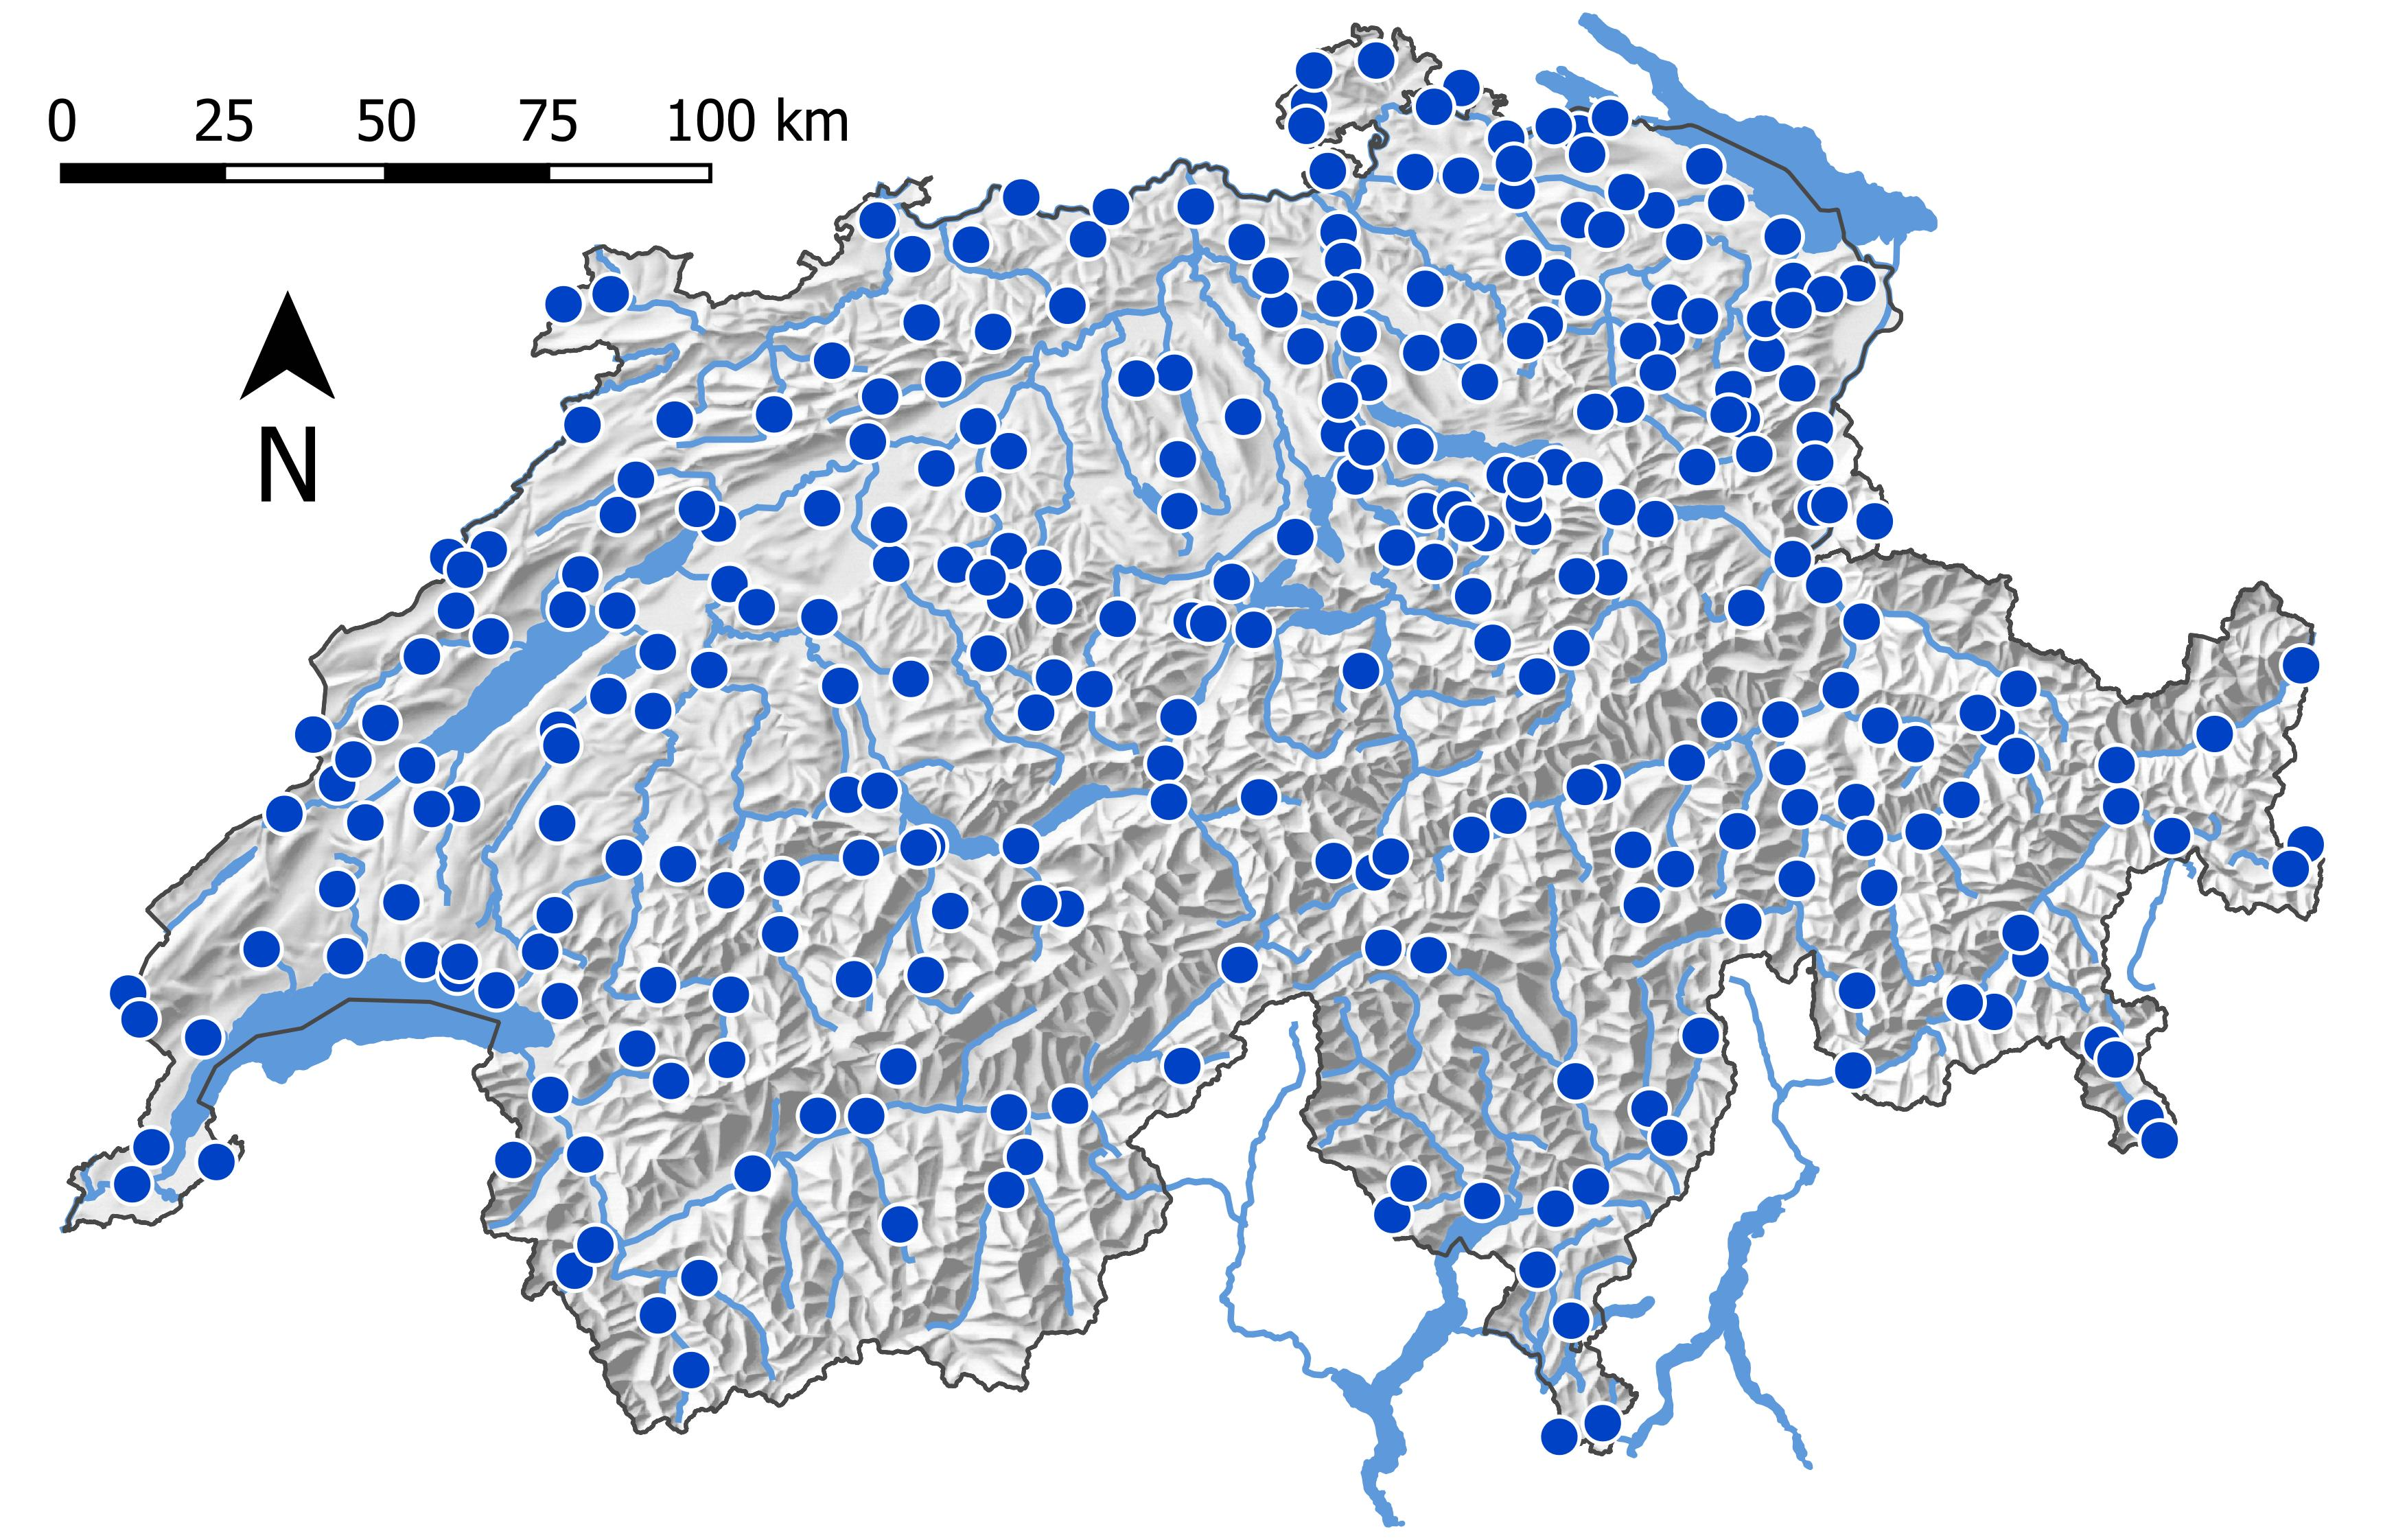
\includegraphics[width=80mm]{figure-1.jpg}\\
	\caption{Map of the 301 precipitation stations with good data coverage of the period 1981--2010. Background map: \textcopyright\ SwissTopo. Modified from \citet{Horton2018b}.}
	\label{fig:stations}
\end{figure}

\begin{figure}[bt]
	\centering
	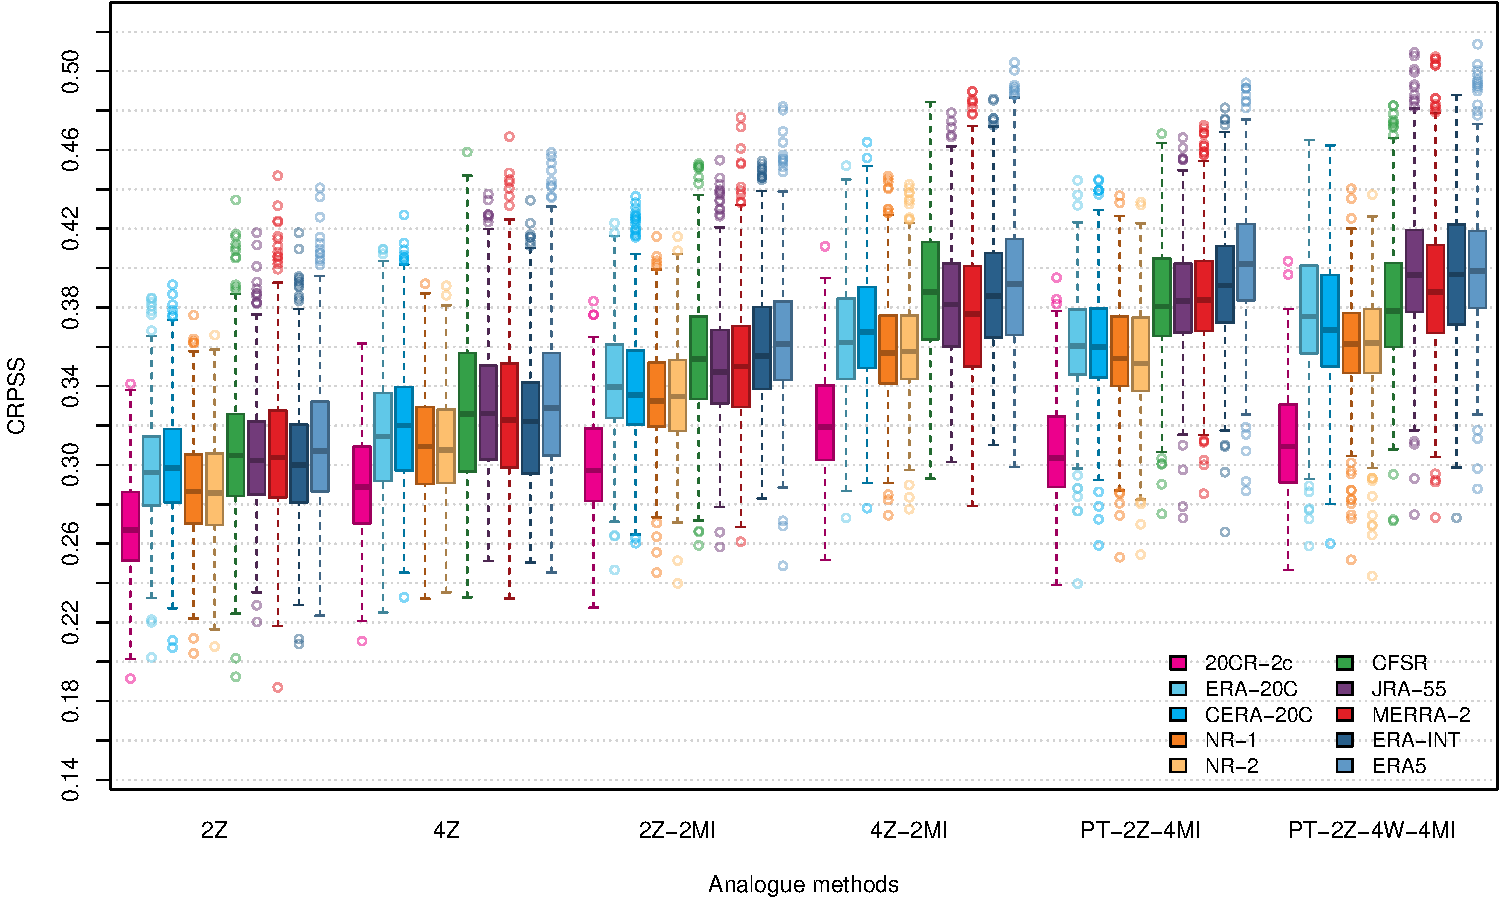
\includegraphics[width=100mm]{figure-2.pdf}
	\caption{Comparison of ERA-INT and ERA5 at 0.25\degree\ and 0.75\degree\ as well as a failed calibration of AMs with ERA5 (gray; named "ERA5 0.25 issues"; see explanation in text). The performance is given by the CRPSS for all stations and all AMs on the VP. The boxes show the 25th, 50th, and 75th percentiles. The whiskers extend to the most extreme data point, which is no more than 1.5 times the interquartile range.}
	\label{fig:resolution}
\end{figure}

\begin{figure}[btp]
	\centering
	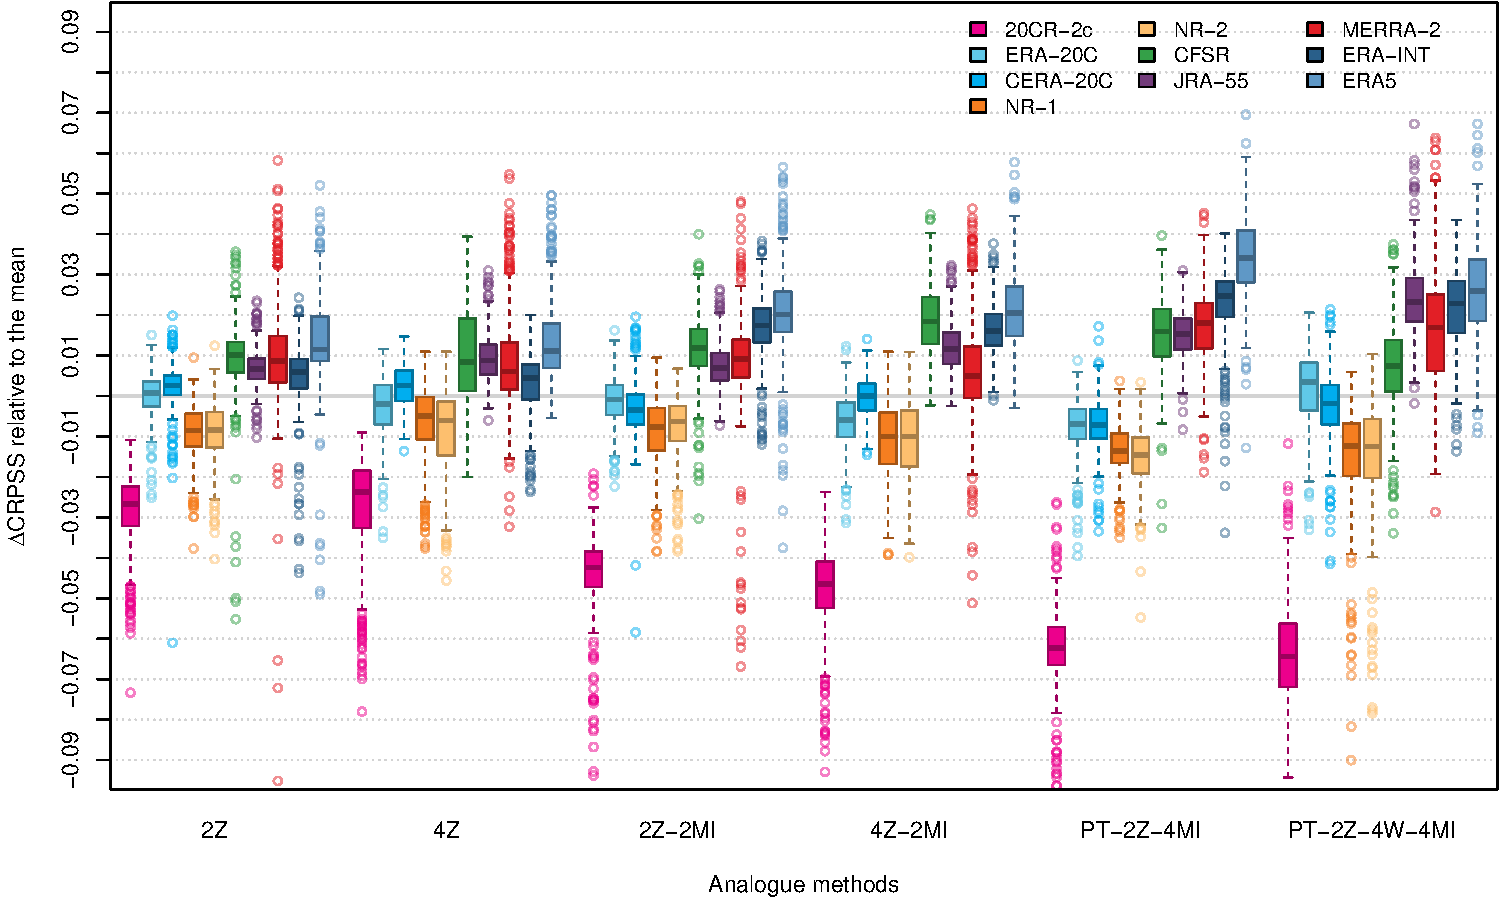
\includegraphics[width=115mm]{figure-3.pdf}
	\caption{Calibrated number of analogs for the different methods and reanalyses, and for all stations. The reanalyses are ordered by increasing spatial resolution. The triangles represent the mean values of all stations.}
	\label{fig:params-nb-analogs}
\end{figure}

\begin{figure}[btp]
	\centering
	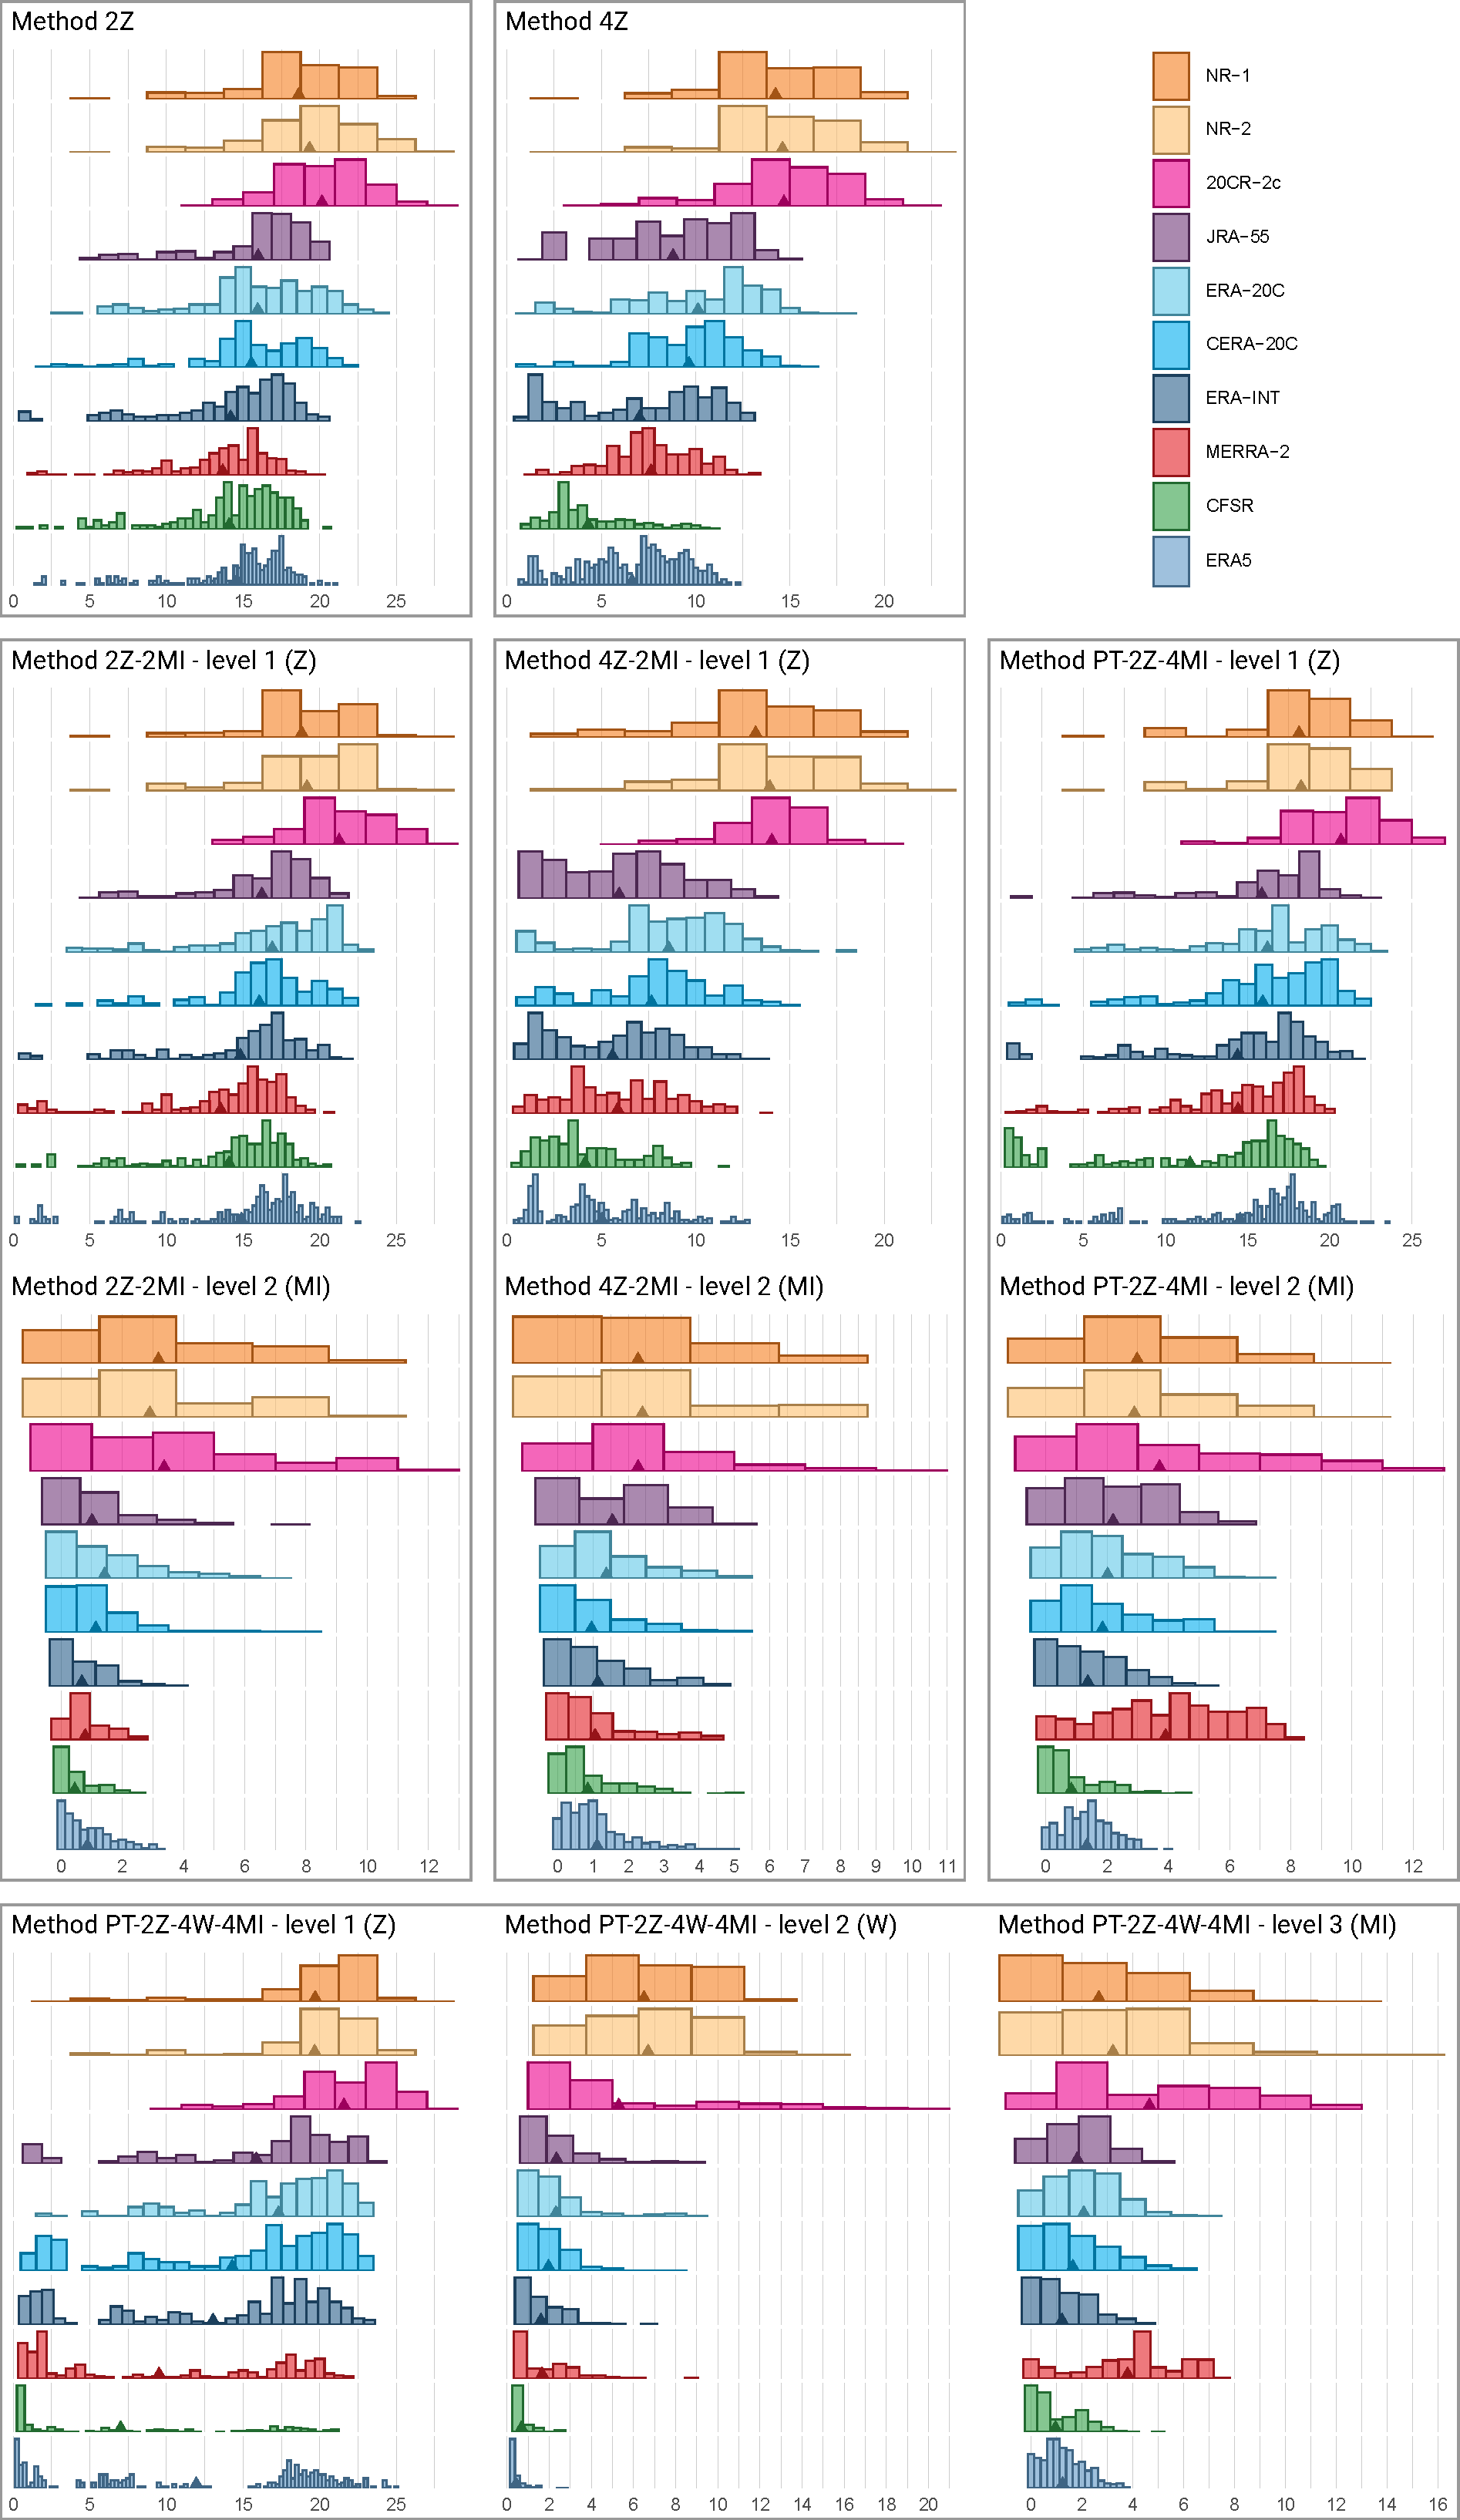
\includegraphics[width=115mm]{figure-4.pdf}
	\caption{Calibrated zonal extents (in degrees) of the spatial windows for the different methods and reanalyses, and for all stations. Same conventions as Fig. \protect\ref{fig:params-nb-analogs}.}
	\label{fig:params-xwidth}
\end{figure}

\begin{figure}[btp]
	\centering
	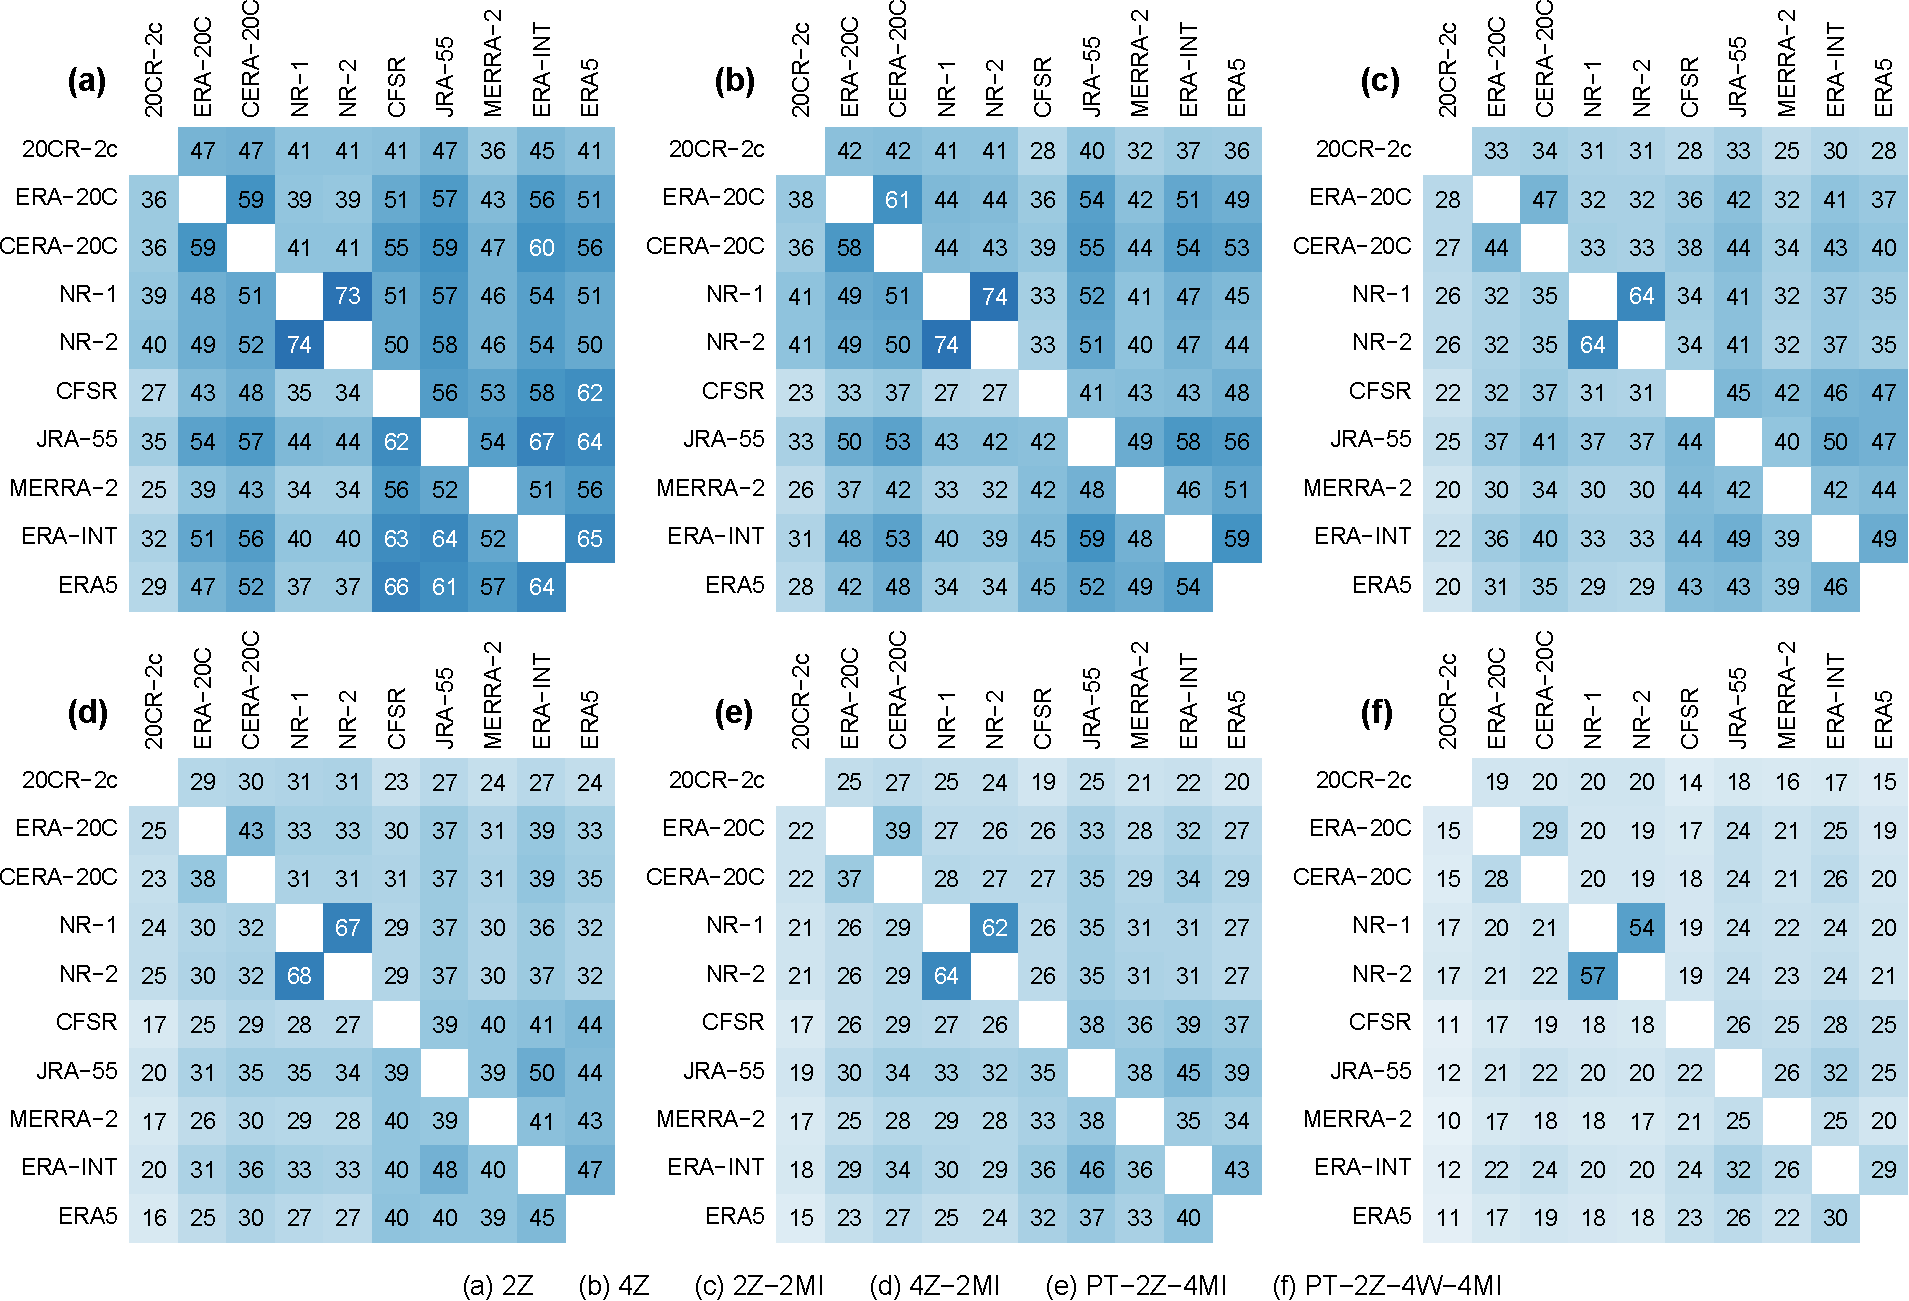
\includegraphics[width=115mm]{figure-5.pdf}
	\caption{Calibrated meridional extents (in degrees) of the spatial windows for the different methods and reanalyses, and for all stations. Same conventions as Fig. \protect\ref{fig:params-nb-analogs}.}
	\label{fig:params-ywidth}
\end{figure}

\begin{figure}[bt]
	\centering
	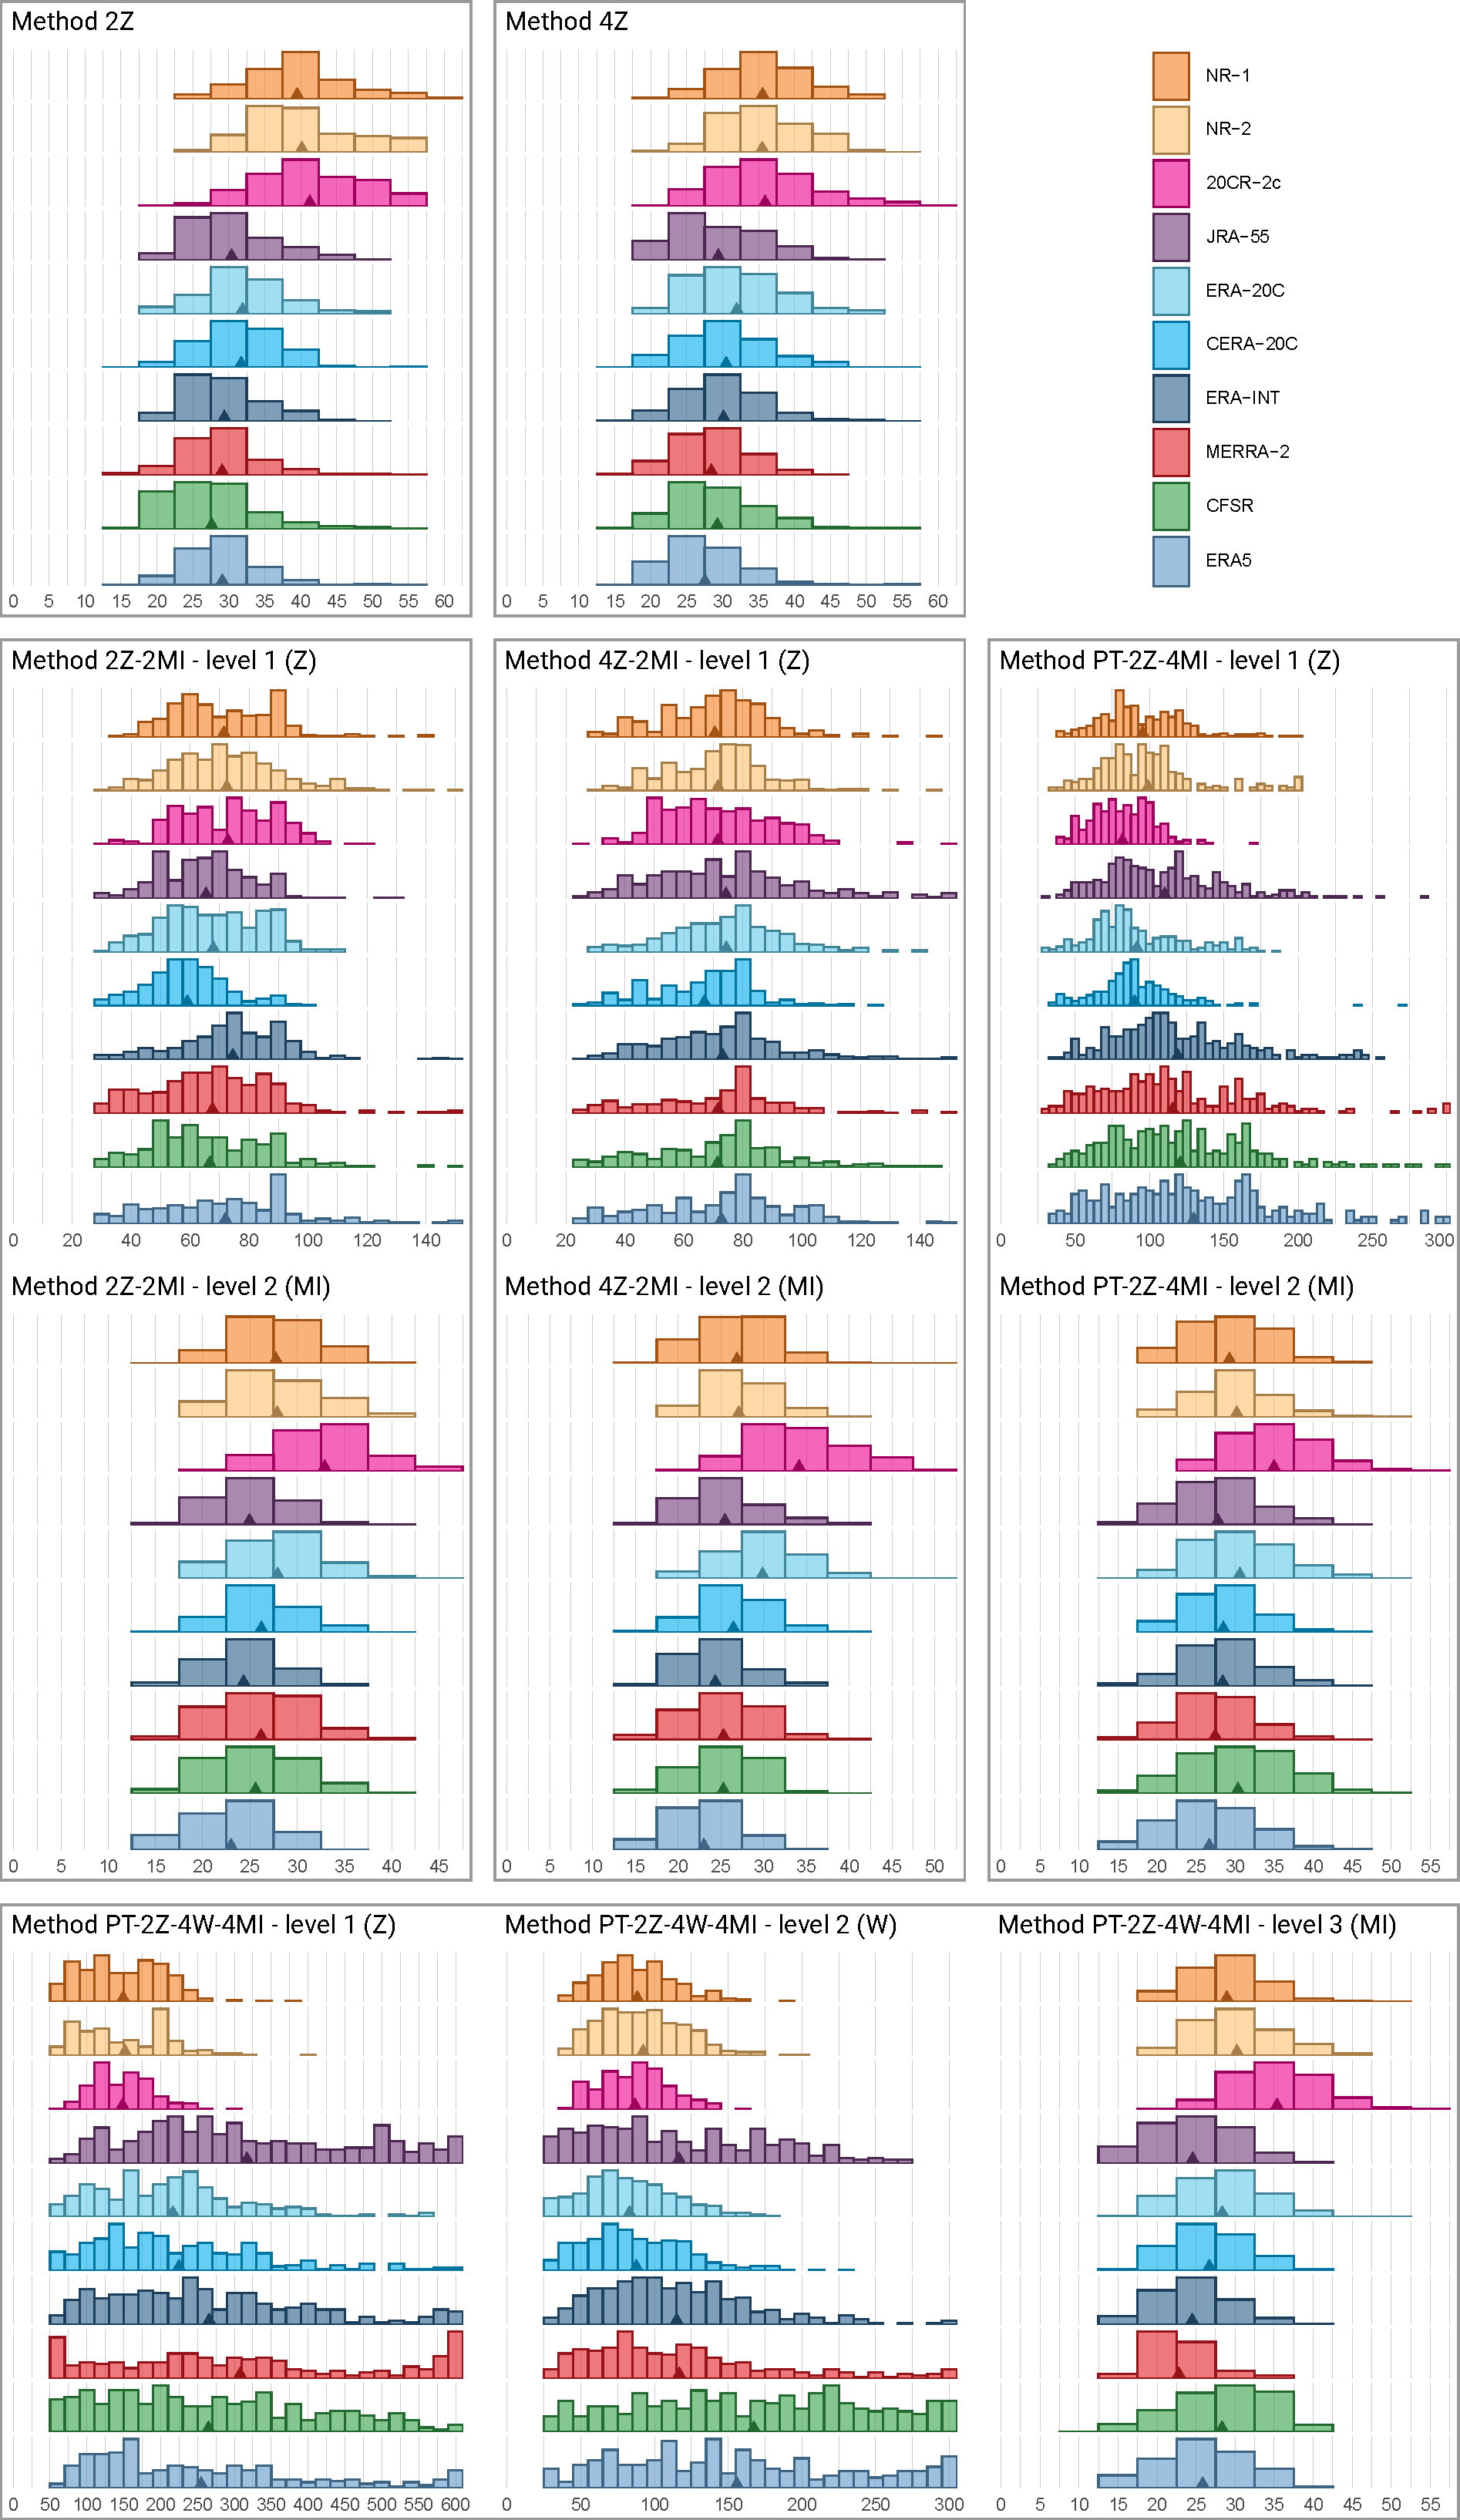
\includegraphics[width=\textwidth]{figure-6.pdf}
	\caption{CRPSS for all stations and all considered AMs and reanalysis datasets on the VP. A higher CRPSS means better performance. The parameters of the AMs were calibrated for every station, dataset, and method. The boxes show the 25th, 50th, and 75th percentiles. The whiskers extend to the most extreme data point, which is no more than 1.5 times the interquartile range.}
	\label{fig:comparison_values}
\end{figure}

\begin{figure}[bt]
	\centering
	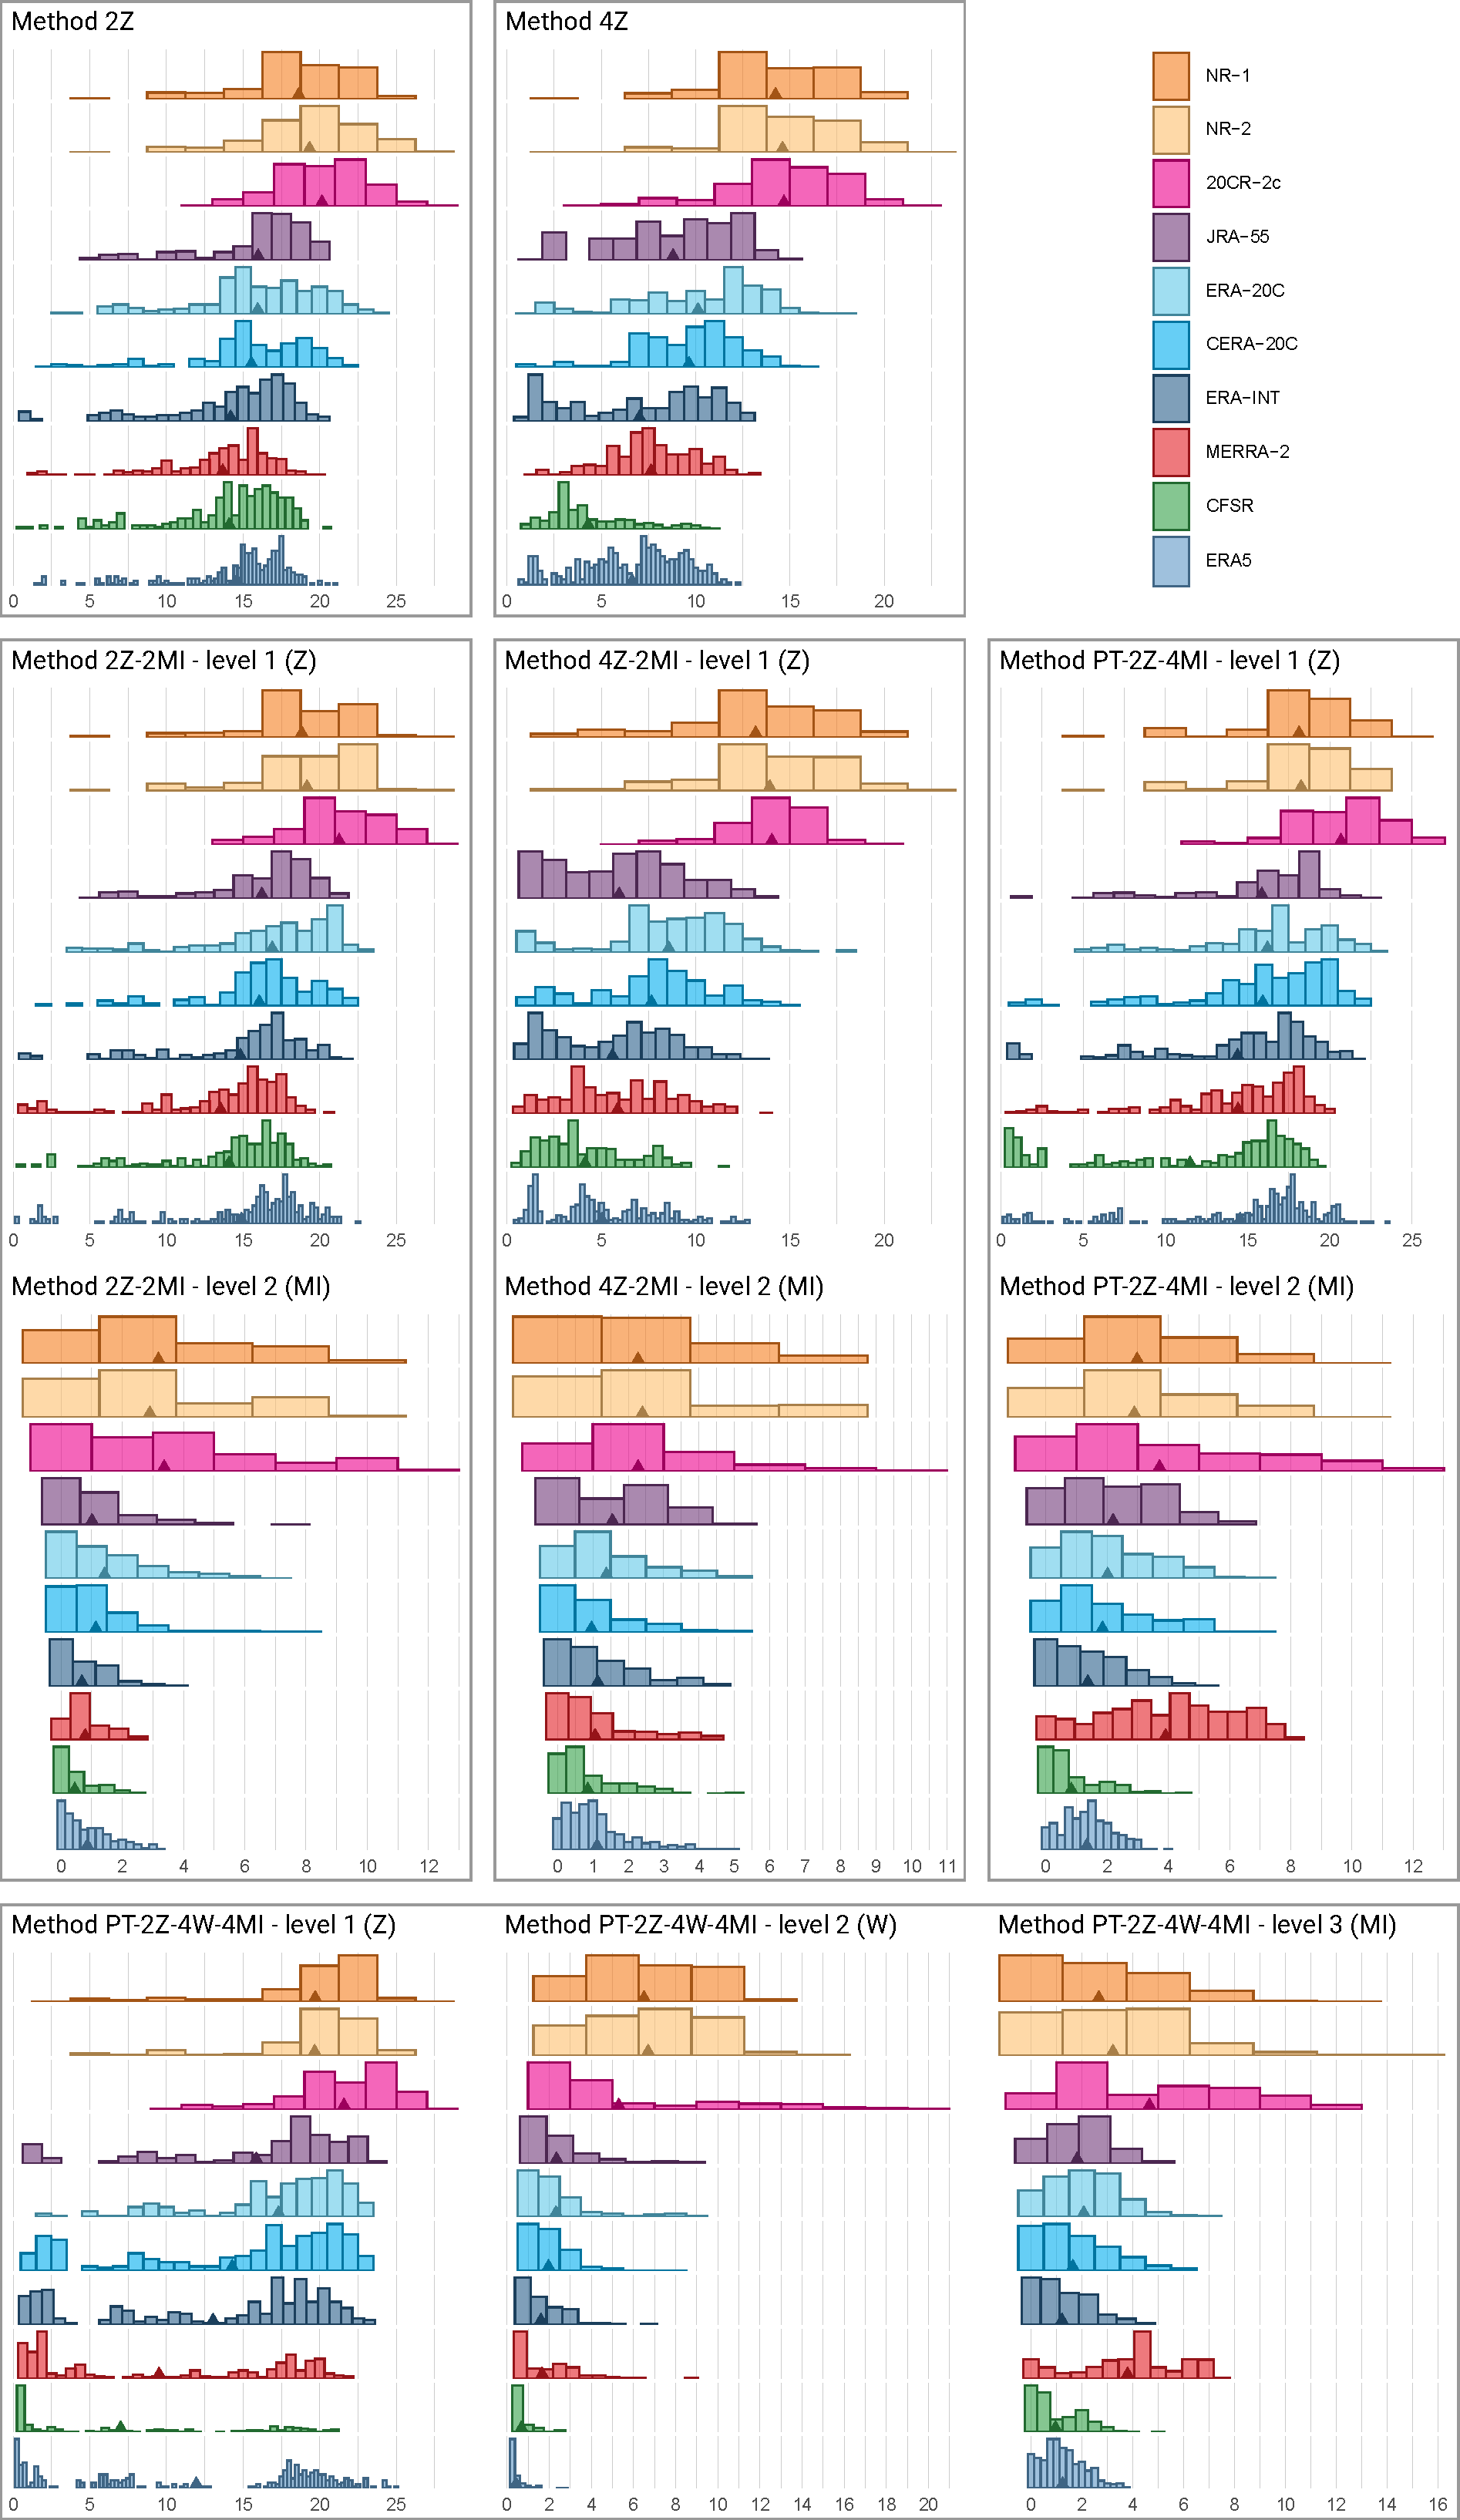
\includegraphics[width=\textwidth]{figure-7.pdf}
	\caption{Impact of the reanalysis dataset on performance, isolated by processing the improvement in CRPSS for one dataset compared to the mean performance on all datasets, per station and method. Note that the methods cannot be compared here, only the datasets. Same conventions as Fig. \protect\ref{fig:comparison_values}.}
	\label{fig:comparison_relative}
\end{figure}

\begin{figure}[bt]
	\centering
	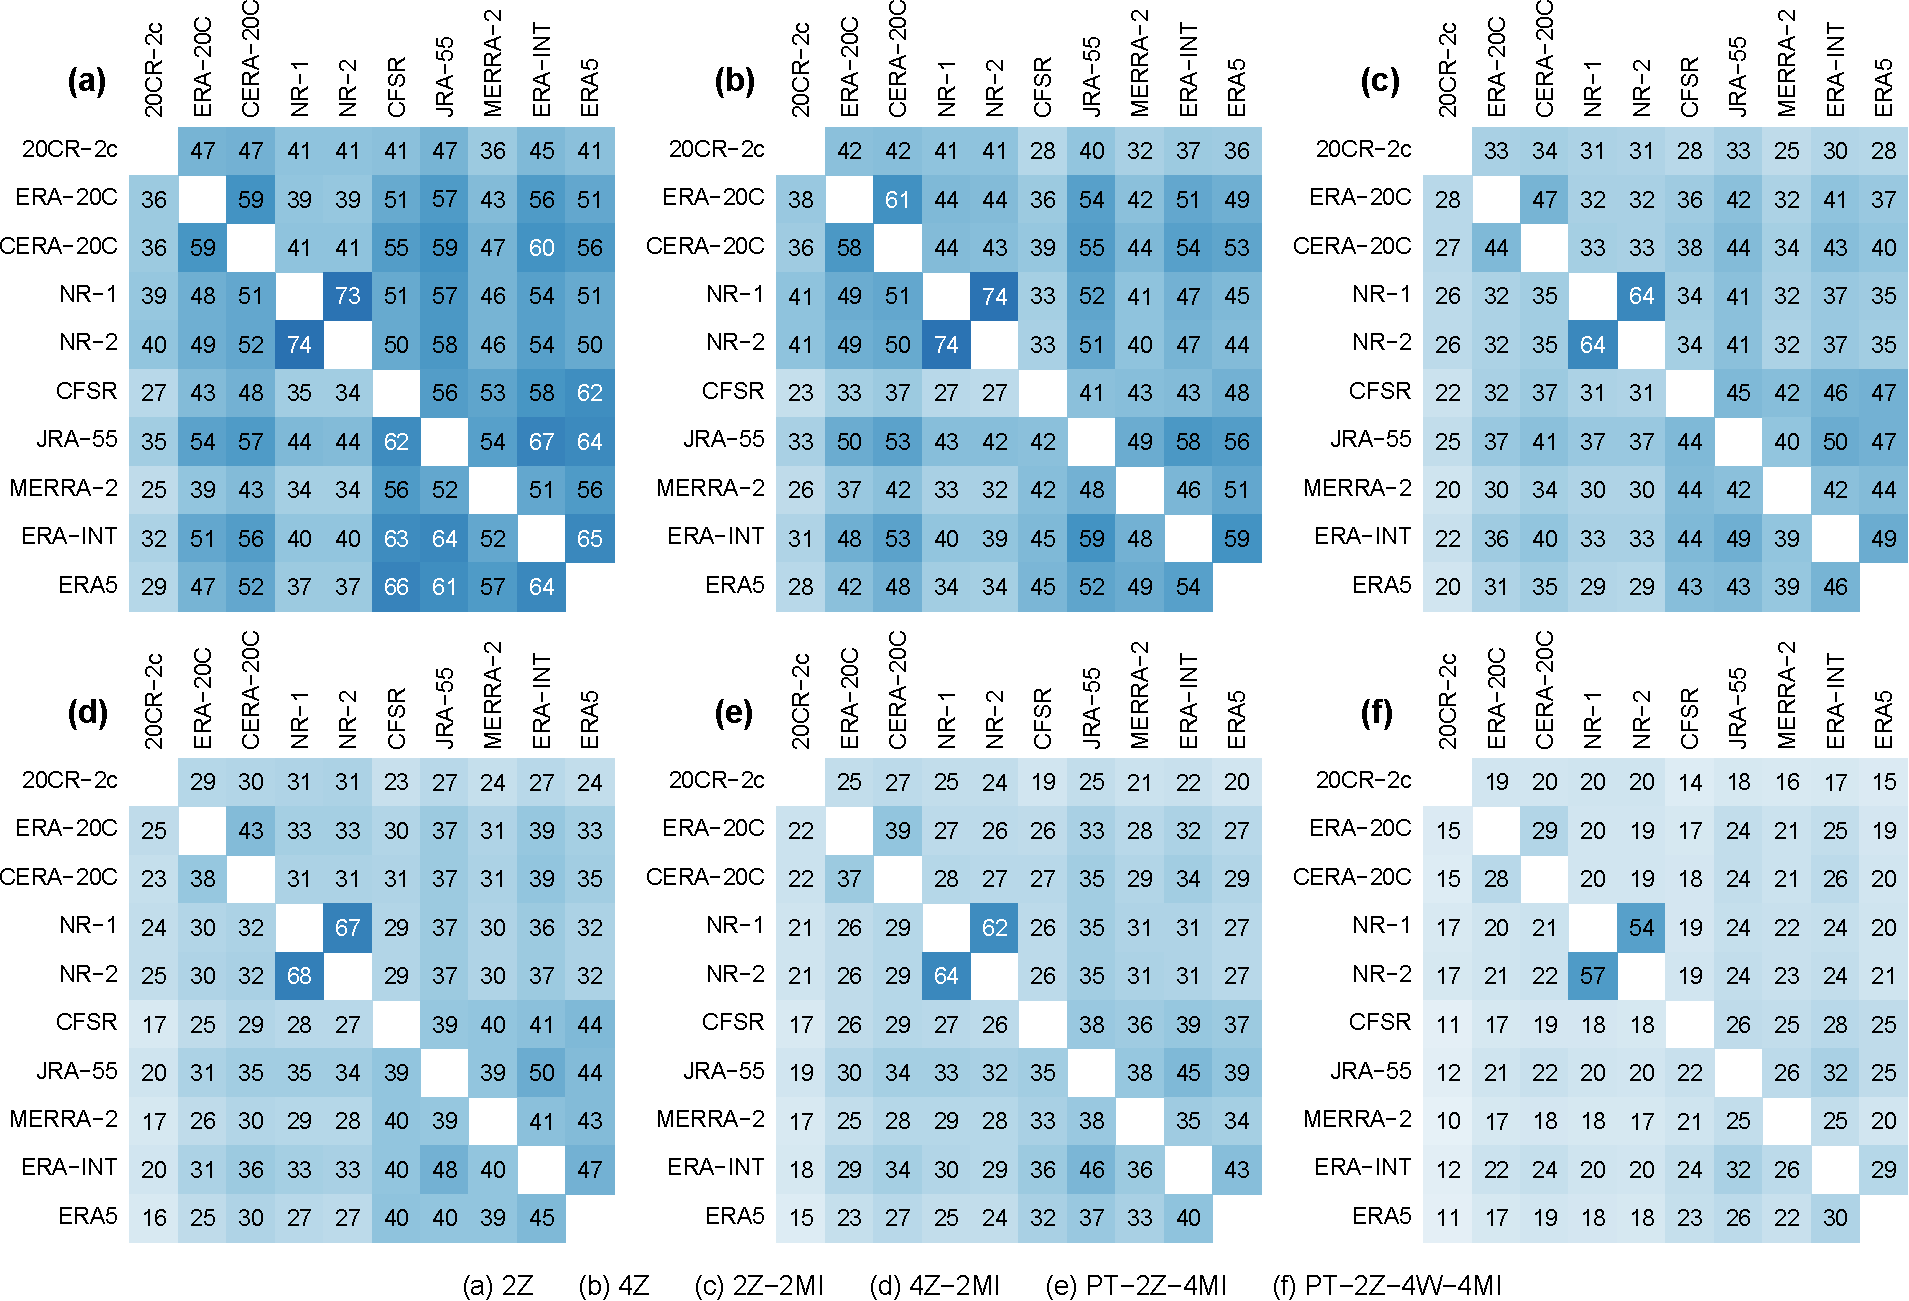
\includegraphics[width=120mm]{figure-8.pdf}
	\caption{Percentage of identical analog dates for different AMs, selected when using the reanalyses in columns that were also found when using the reanalyses in rows. The values were averaged for all stations on the VP.}
	\label{fig:shared-dates}
\end{figure}



\end{document}
